\section{Stand der Technik}

In diesem Abschnitt wird der Stand der Technik in den Bereichen Messtechnik, ausgewählter verfahrenstechnischer Prozesse, digitale Schnittstellen und Signalverarbeitung sowie Datenverwaltung, in Bezug auf die \textit{digitale Transformation} des VT-Labors, erläutert. 

%\subsection{Messtechnik}

In diesem Abschnitt werden ausgewählte analoge und digitale Druck- und Volumenstrommesstechniken erläutert, die in Laboren anwendung finden.

\subsubsection{Gas Durchflussmessung}

Den Durchfluss eines Mediums in einer geschlossenen Rohrleitung lässt sich mit verschiedenen Messprinzipien bestimmen. Zu den Volumendurchflussmessungen gehören z.B. die:

\begin{itemize}
\item Ultraschalldurchflussmessung
\item Wirkdruckverfahren
\item Schwebekörperdurchflussmesser
\end{itemize}

und zu den Massendurchflussmessprinzipien zählen z.B. die:

\begin{itemize}
\item thermische Massendurchflussmessung
\item Coriolis Durchflussmessung
\item Mikromechanische Flusssensormessung
\end{itemize}

%\paragraph{Volumendurchflussmessung}

%\subparagraph{Wirkdruckverfahren}

%\subparagraph{Ultraschalldurchflussmessung}

\paragraph{Massendurchflussmessung}

Mittels der 

\subparagraph{Coriolis}

Massendurchflussmesser mini CORI-FLOW™ series

\subparagraph{thermische Massendurchflussmessung}

Die Durchflussmessung von Gasen ist mittels thermischen Massendurchflussmesser möglich. Zur Messung des Massendurchflusses wird die Wärmeleitfähigkeit von Fluiden genutzt. Der prinzipielle Aufbau so eines Sensors ist in Abbildung \ref{MFC} dargestellt.

\bild{0.5}
{MFC.png}
{0em}
{Prinzip eines thermischen Massendurchflussensors}
{Prinzip eines thermischen Massendurchflussensors}
{MFC}

 Im inneren des Durchflussmessers sind zwei Temperatursensoren verbaut. Ein Sensor befindet sich nicht direkt im Strömungskanal (in einem Sackloch) und misst die Veränderung der Umgebungstemperatur $T_U$, als auch die Wärmeübertragung des Fluids als Referenz. Der zweite Sensor wird beheizt. Die Temperaturdifferenz $\Delta T$ wird konstant gehalten. Je höher die Fließgeschwindigkeit des Mediums, desto mehr Energie muss dem zweiten Sensor zugeführt werden, um die Temperaturdifferenz konstant zu halten.  Der Massenstrom $\dot{m}$ ist dem Wärmestrom $\dot{Q}$ proportional. Es gilt folgender Zusammenhang zwischen Massen- und Wärmestrom:

\begin{align}
\dot{Q}=\dot{m} \cdot c_p \cdot  \Delta T
\end{align}

Der Massenstrom ist der zugeführten Energie in Form von Strom $I^2$ proportional. Der zweite Sensor hat einen Temperaturabhängigen Widerstand $R(T)$. 

\begin{align}
\dot{m}=\dfrac{R(T) \cdot I^2}{c_p \cdot \Delta T}
\end{align}

Beide Sensoren sind zu einer Wheatstone'schen Messbrücke verschaltet, $\sqrt{\dot{m}}$ ist der Ausgangsspannung $\Delta U_Br$ proportional .

\subsubsection{Druckmessung}


\subsection{Messtechnik}

In diesem Abschnitt werden ausgewählte digitale Druck- und Volumenstrommesstechniken aufgezeigt, die in Laboren Anwendung finden. 

\subsubsection{Digitale Durchflussmesstechnik für Gase}
\label{sec:digi_durchfluss}

Zum messen von Durchflüssen oder Mengen gibt es eine Vielzahl von Verfahren. In der Abbildung \ref{fig:durchfluss_messverfahren} ist eine Übersicht der verschiedenen Messverfahren abgebildet. Nicht alle Messverfahren der Abbildung \ref{fig:durchfluss_messverfahren} sind dafür geeignet, um Volumen- oder Massenströme von Gasen zu messen. Auf die Messprinzipien aller Sensoren dieses Abschnitts wird im Rahmen dieser Arbeit nicht eingegangen. Für tiefgreifende Informationen wird auf Fachliteratur, wie z.B. \cite{Stiess2008, Tränkler2015, Wiegleb2016, SensorTechnologien} verwiesen. Messprinzipien, die für die Messung von Luft geeignet sind und in Sensoren ihre Anwendung finden, sind die folgenden: 

\begin{figure}[h!]
\vspace{-1em}
\centering
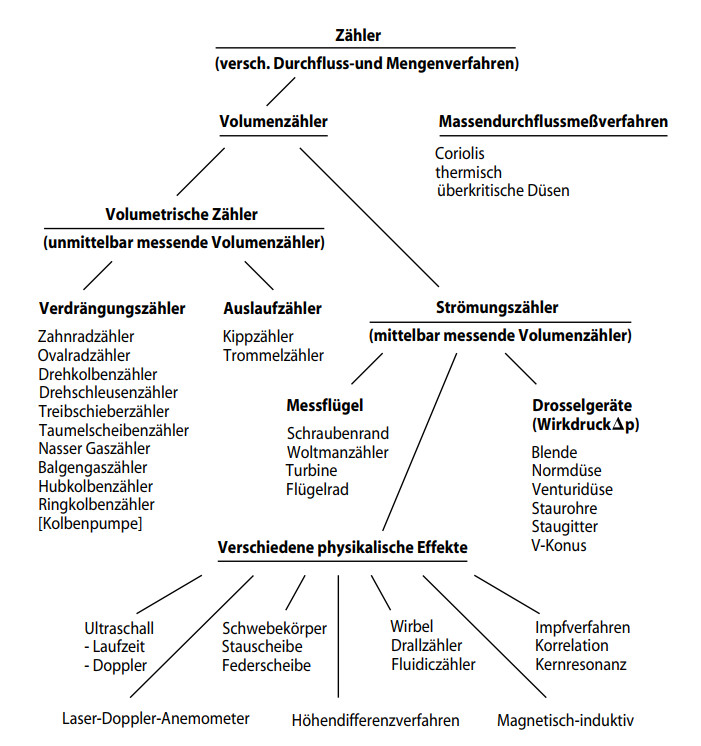
\includegraphics[width=0.75\textwidth]{Bilder/versch_Durchflussmess-Mengenverfahren.jpg}
\caption{Übersicht verschiedener Durchfluss- und Mengenmessverfahren \cite[S. 794]{SensorTechnologien}}
\label{fig:durchfluss_messverfahren} 
\end{figure}




\begin{itemize}
\singlespacing
\item \glqq Kraft auf Körper\grqq{} Durchflussmessung (Volumenstrom, non-digital)
\item Differenzdruckverfahren (Volumenstrom)
\begin{itemize}
\item Lochblende
\item Venturi-Rohr
\end{itemize}
\item Vortexdurchflußmessung (Volumenstrom, für Gase nur in Kombination mit Dichtemessung Massenstrom)
\item thermische Massendurchflussmessung (Massenstrom)
\item Coriolis Durchflussmessung (Massenstrom)
\end{itemize}

\paragraph*{Kraft auf Körper Durchflussmessung} Da ein Versuchsstand im Rahmen dieser Arbeit, zu Beginn des Projekts, einen (\textit{analog}) \textbf{S}chwebe\textbf{k}örper\textbf{d}urchfluss\textbf{m}esser (SKDM; siehe Abbildung \ref{fig:mech_durchflussmesser}) besitzt und eine diversitäre Redundanz, mittels \textit{digitalem} Sensor, erfolgen soll, wird das Wirkprinzip dieses rein analogen Messverfahrens erläutert. Gemäß \cite[S. 827 ff.]{Tränkler2015} wird dieses Messverfahren \glqq Kraft auf Körper genannt\grqq. Ein \textit{Festkörper} wird in einer konischen Rohrleitung angeströmt und wird angehoben oder ausgelenkt, im Falle eines \textbf{Federscheibendurchflussmessers}, bei hinreichend großer Anströmgeschwindigkeit. Eine äquivalente Lösung, ist dass installieren eines  konischen Schwebekörper in eine Blendenöffnung. Sobald sich ein Kräftegleichgewicht einstellt, verharrt der Festkörper in der Position. Die geometrischen Formen der Festkörper können z.B. ein Konus (SKDM) oder eine Scheibe (Federscheibendurchflussmessers) sein \cite[S. 827]{Tränkler2015}. Der abzulesende Volumenstrom ist somit unter anderem eine Funktion des durchströmten Querschnitts $A$. Das physikalische Wirkprinzip ist ein Kräftegleichgewicht. Wenn sich die Gravitationskraft $F_\mathrm{G}$, abzüglich der Auftriebskraft $F_\mathrm{A}$ eines Partikels oder Festkörpers, mit der Widerstandskraft $F_\mathrm{W}$ im Gleich\-gewicht befindet (siehe Gleichung \ref{eq:gleichgewicht}), dann befindet sich die Strömung in einem stationärem Zustand. Für ein frei bewegliches Festkörperpartikel, welches sich im Gravitationsfeld befindet und vertikal von unten angeströmt wird (z.B. SKDM), gilt Gleichung \ref{eq:gleichgewicht} \cite[S. 105 ff.]{Stiess2008}.

\begin{align}
\label{eq:gleichgewicht}
F_\mathrm{G} - F_\mathrm{A} = F_\mathrm{W}
\end{align}

Die Widerstandskraft $F_\mathrm{W}$ eines Festkörpers in einer Strömung lautet:

\begin{align}
\vec{F}_\mathrm{W} = c_\mathrm{w} (\mathrm{Re}_x) \cdot A \cdot \rho_\mathrm{f} \cdot \frac{\vec{v} \cdot \vert v\vert}{2}
\end{align}

Der $c_\mathrm{w}$ Wert gibt den Widerstand eines Partikels in einer Strömung an. Er ist abhängig von der Form sowie Größe eines Partikels (Index $x$) und ist eine Funktion der Reynoldszahl.\\

\paragraph*{Differenzdruckbasierte Sensoren} Differenzdruckbasierte Sensoren sind robust, bieten eine hohe Prozesssicherheit und sind kostengünstig. Sie
eignen sich besonders für große Durchflussmengen. Dieses Verfahren wird auch Wirkdruckverfahren genannt. Die Nutzung einer \textbf{Lochblende} hat den Vorteil, dass ein großer Messbereich, durch Wechsel bzw. Variation der Lochblende, genauer Durchflussöffnung, realisierbar ist. Für den Betrieb eines differenzdruckbasierten Sensors mittels Lochblende ist zu beachten, dass durch die Drosselung  und die dadurch auftretende Dissipation von Energie, hohe Betriebskosten entstehen können.
\textbf{Venturi-Rohre} haben eine bessere Energiebilanz gegenüber Lochblenden. Des Weiteren weisen Venturi-Rohre gegenüber Lochblenden weniger Verschleiß  auf und sind demnach weniger Wartungsintensiv \cite[S. 823 ff.]{Tränkler2015}.


\paragraph*{Sensoren auf Basis der Corioliskraft} Um den Massenstom von Fluiden zu ermitteln, kann sich die, aus dem zweiten newtonschen Axiom hergeleitete, Corioliskraft zu nutze gemacht werden. Die Corioliskraft ist, wie die Zentrifugalkraft, eine Scheinkraft. Die Corioliskraft ($ \vec{F}_c=f(\vec{a}_\mathrm{c}$)\,), zur Bestimmung des Massendurchflusses, ist proportional zur Masse des durchströmten Messrohrs ($\vec{F}_\mathrm{c}=m \cdot \vec{a}_\mathrm{c}$), in der Abbildung \ref{fig:coriolisod} und \ref{fig:coriolisd} ist es das U-Rohr. Das Messrohr wird elektromagnetisch in Schwingung gesetzt. Wird das Messrohr durchströmt, tritt der Coriolis-Effekt auf und das Messrohr oszilliert um die y-Achse (siehe Abbildung \ref{fig:coriolisd}). Für tiefgreifendes Wissen zum Wirkprinzip des Sensors muss auf Fachliteratur verwiesen werden \cite[S. 268 ff.]{SensorTechnologien}.

\begin{figure}[p!] 
\centering
%\hspace{0em}
%\captionsetup{position=top}

     \subfloat[][Schwebekörperdurchflussmesser~(\texttt{links}) \newline Federscheibendurchflussmesser~(\texttt{rechts})\label{fig:mech_durchflussmesser}]{%
       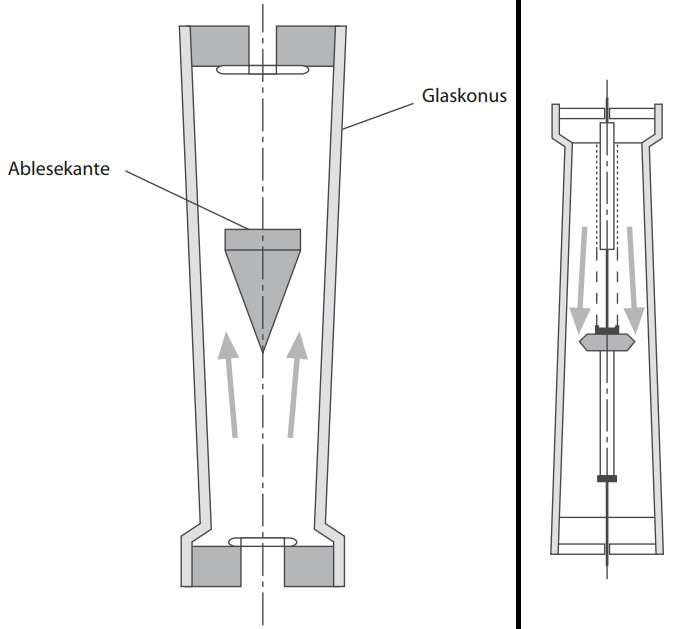
\includegraphics[width=0.40\textwidth]
       {Bilder/mechanische_durchflussmesser.jpg} %{Bilder/LabVIEW_serialport/}
     }%\hspace{-1.5pt}%
     \hfill     
    \subfloat[][Wirkdruckdrosselgeräte Übersicht nach DIN\label{fig:Wirkdruckverfahren}]{%
       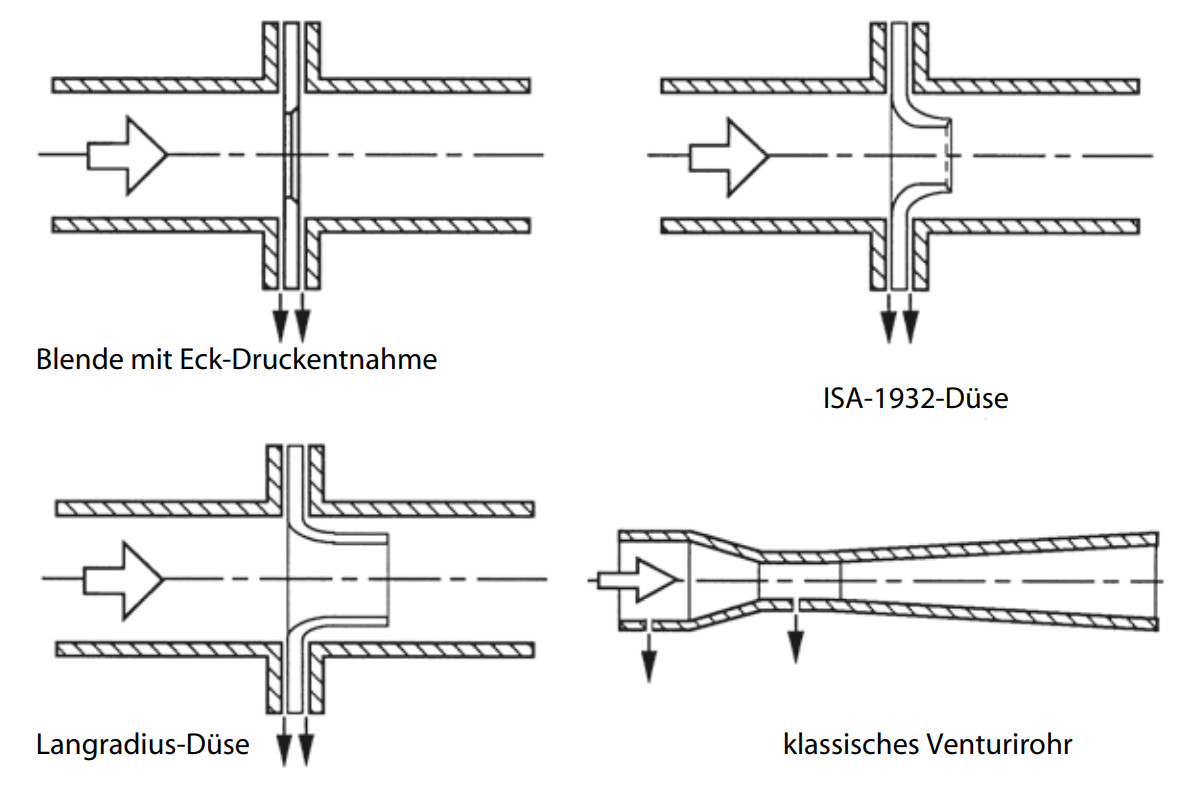
\includegraphics[width=0.45\textwidth]
      {Bilder/Wirkdruckverfahren.jpg}
     }\phantomcaption
%\vspace{-.81em}
\ContinuedFloat

     \subfloat[][angeregter Coriolissensor ohne Durchsatz\label{fig:coriolisod}]{%
       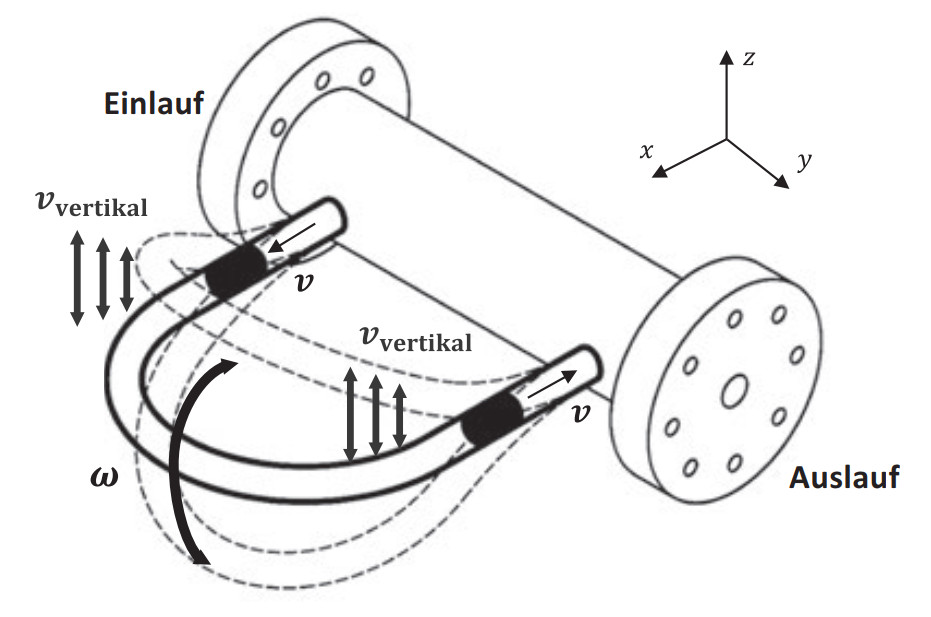
\includegraphics[width=0.45\textwidth]
       {Bilder/coriolis_leer.jpg} %{Bilder/LabVIEW_serialport/}
     }%\hspace{-1.5pt}%
     \hfill     
    \subfloat[][angeregter Coriolissensor mit Durchsatz\label{fig:coriolisd}]{%
       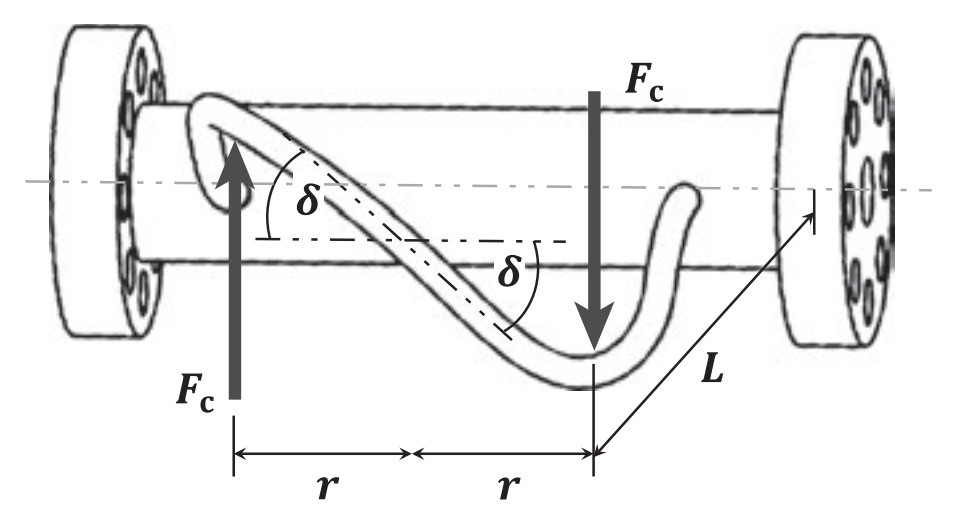
\includegraphics[width=0.45\textwidth]
      {Bilder/coriolis_durchsatz.jpg}
     }\phantomcaption
%\vspace{-.81em}
\ContinuedFloat
\captionsetup{position=bottom}
\subfloat[position=top][Vortexsensor\label{fig:vortexsensor}]{%
       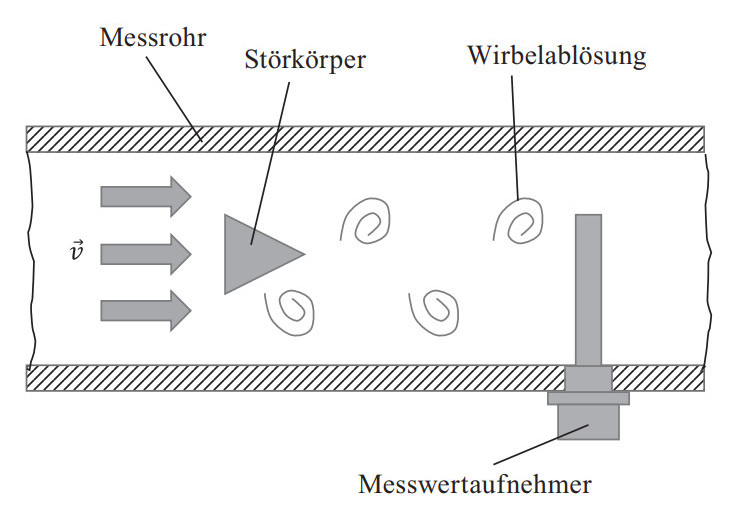
\includegraphics[width=0.45\textwidth]
       {Bilder/vortexsensor.jpg}
     }%\hspace{-1.6pt}%
     \hfill     
    \subfloat[position=top][Drallsensor \label{fig:drallsensor}]{%
       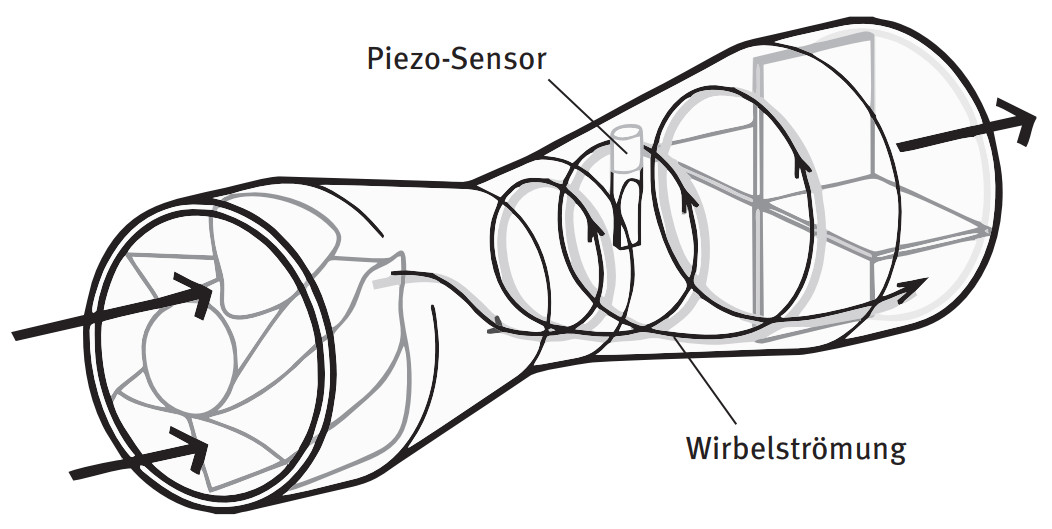
\includegraphics[width=0.45\textwidth]
      {Bilder/drallsensor.jpg} %{Bilder/LabVIEW_serialport/}
     }    
\caption[Übersicht einiger Sensoren, die für die Messung von Gasdurchflüssen geeignet ist]
{Übersicht einiger Sensoren, die für die Messung von Gasdurchflüssen geeignet ist:
(a) Mechanische Durchflusssensoren
(b) Wirkdruckverfahren \cite[S. 826]{Tränkler2015},
(c, d) Coriolisensor \cite[S. 270]{SensorTechnologien}
(e, f) Vortex- sowie Drallsensor}
\label{fig:Sensorübersicht}
   \end{figure} 

\paragraph*{Vortexdurchflusssensoren} Die industrielle Nutzung von Vortexdurchflußsensoren (Wirbelsensoren, siehe Abbildung \ref{fig:vortexsensor}) begann in den 1960er-Jahren.  Das physikalische Grundprinzip ist die Kármánsche Wirbelstraße. Das Wirkprinzip beruht auf der Anregung eines Störkörpers, wie eines Drahtes, in einer Strömung. Die Schwingfrequenz ist proportional zur Anströmgeschwindigkeit und antiproportional zur Dicke des Drahtes. Die Ursache der Schwingung ist die Wirbelablösung hinter einem Strömungswiderstand. Die Geometrie des Störkörpers beeinflusst die Wirbelbildung und somit die Schwingung maßgeblich. Bei der Durchflussbestimmung von Gasen ist eine Sensornahe Bestimmung der Dichte erforderlich, da durch die Kompressibilität von Gasen, Dichtedifferenzen auftreten können, die sich maßgeblich auf die gemessene Durchsatzmenge auswirken. Für Gase ist der Vortexsensor, durch die Kombination mit einer Dichtemessung, somit nur als Massendurchflusssensor geeignet. Eine Weiterentwicklung des Vortexdurchflussensors ist der Drallsensor (siehe Abbildung \ref{fig:drallsensor}). Durch den induzierten Drall kann die Einlaufstrecke signifikant verkürzt werden \cite[S. 294 ff.]{SensorTechnologien}.




\paragraph{Thermischer Massendurchflusssensor}

Die Durchflussmessung von Gasen ist mittels thermischen Massendurchflussmesser möglich. Zur Messung des Massendurchflusses wird die Wärmeleitfähigkeit des zu messenden Fluids genutzt. Der prinzipielle Aufbau so eines Sensors ist in Abbildung \ref{MFC} dargestellt.

\bild{0.45}
{MFC.jpg}
{0em}
{Prinzip eines thermischen Massendurchflussensors}
{Prinzip eines thermischen Massendurchflussensors \cite[S. 656]{Wiegleb2016}}
{MFC}

Auf das Messprinzip dieses Sensors wird genauer eingegangen, da er im Rahmen dieses Projekts und in den folgenden Praxisveranstaltungen verwendet wird. Im Inneren des Durchflussmessers sind zwei Temperatursensoren verbaut. Ein Sensor befindet sich nicht direkt im Strömungskanal (in einem Sackloch) und misst die Veränderung der Umgebungstemperatur $T_\mathrm{U}$, als auch die Wärmeübertragung des Fluids als Referenz. Der zweite Sensor wird beheizt. Die Temperaturdifferenz $\Delta T$ wird konstant gehalten. Je höher die Fließgeschwindigkeit des Mediums, desto mehr Energie muss dem zweiten Sensor zugeführt werden, um die Temperaturdifferenz konstant zu halten.  Der Massenstrom $\dot{m}$ ist dem Wärmestrom $\dot{Q}$ proportional. Es gilt folgender Zusammenhang zwischen Massen- und Wärmestrom:

\begin{align}
\dot{Q}=\dot{m} \cdot c_\mathrm{p} \cdot  \Delta T
\end{align}

Der Massenstrom ist der zugeführten Energie in Form von Strom $I^2$ proportional. Der zweite Sensor hat einen temperaturabhängigen Widerstand $R(T)$. 

\begin{align}
\dot{m}=\dfrac{R(T) \cdot I^2}{c_\mathrm{p} \cdot \Delta T}
\end{align}

Beide Sensoren sind zu einer Wheatstone'schen Messbrücke verschaltet, $\sqrt{\dot{m}}$ ist der Ausgangsspannung $\Delta U_{\mathrm{Br}}$ proportional \cite[S. 656]{Wiegleb2016}.

\vspace{2em} 

\subsubsection{Druckmessung}

In der Industrie ist die Bestimmung von Drücken eine fundamentale Messoperation. Bis in die sechziger Jahren wurde der Druck in der Industrie mittels mechanischen Manometern bestimmt. Diese Technologie wurde daraufhin von den sog. Druckaufnehmern, mittels \textbf{D}ehnungs\textbf{m}ess\textbf{s}treifen (DMS) des Werkstoffs Metall oder Drucksensoren, unter der Verwendung von Halbmetallen, abgelöst.  

\paragraph*{Dehnungsresistive Sensoren}

Drucksensoren mittels DMS sind sog. \textit{dehnungsresistive} Drucksensoren. Dehnungsresistive Sensoren nutzen elektrisch Leitende Werkstoffe bzw. Metalle. Das Messprinzip beruht auf der Änderung des elektrischen Widerstandes $R$, eines elektrisch leitenden Werkstoffs, als Folge einer mechanischen Verformung. Es existieren drei Drucksensortechnologien auf Metallbasis.

\begin{enumerate}[label = \textbullet , itemsep = -0.1em]
\item \textcolor{black!60}{DMS aus Draht} 
\item Metallfolien-DMS
\item Dünnfilm-DMS
\end{enumerate}

In den Jahren von 1938 bis zum Ende der 50er Jahre bestand der DMS aus einem Draht, der mäanderförmig auf einen Dehnkörper aufgebracht wurde. Der Draht wurde von Metallfolien und später Dünnfilm-DMS \textcolor{black!60}{abgelöst} \cite[S. 434]{Tränkler2015}. Zur Erläuterung des physikalischen Wirkprinzips wird als Modell ein zylinderförmiger Körper genutzt. 

%\begin{figure}[h!]
%\centering
%\includegraphics[0.9\textwidth]{Bilder/drahtmodell.jpg}
%\caption{Drahtmodell zur Herleitung des Wirkprinzips}
%\label{fig:drahtmodell} 
%\end{figure}

\subparagraph*{Zylindermodell} Ein zylinderförmiger, elektrisch leitender Werkstoff, charakterisiert durch die Ausgangslänge $l_\mathrm{0}$, Ausgangsquerschnitt $A_\mathrm{0}$ und dem spezifischem elektrischem Widerstand $\rho_{\mathrm{el}}$, hat einen elektrischen Widerstand R gemäß folgender Gleichung \cite[S. 4 ff.]{Wolff2016}:

\begin{align}
\label{eq:zyl_wiederstand}
R=\rho_{\mathrm{el}} \cdot \frac{l_\mathrm{0}}{A_\mathrm{0}}
\end{align}

Von diesem Modell ausgehend wird die relative Widerstandsänderung $\Delta R / R$, durch die Bildung des totalen Differenzials, berechnet. Die Lösung der Differenzialgleichung, gemäß \cite[S. 7 ff.]{Wolff2016} (siehe Anhang Gleichung (\ref{eq:totaldif_dms}), unter der Definition einiger Randbedingungen, führt zur Gleichung (\ref{eq:delta}). 
%
%
%\begin{align}  
%\label{eq:totaldif_dms}
%	dR &=\frac{\partial R}{\partial \rho_{el}} \: d\rho_{el}+\frac{\partial R}{\partial l_0} \: dl_0+\frac{\partial R}{\partial A} \: dA \\[1em]
%		&= \frac{l_0}{A} ~ d\rho_{el} + \frac{\rho_{el}}{A} \: dl_0 - \frac{\rho_{el} \cdot l_0}{A^2} \: dA \\[1em]
%		&= R \cdot ( \frac{d\rho}{\rho} + \frac{dl_0}{l_0} - \frac{dA}{A} )
%\end{align}
%
%
%Ersetzt man das Infinitisimal $d$ durch eine eine größere Schrittweite $\Delta$, unter der Bedingung dass $\Delta \rho \ll \rho,\, \Delta l_0 \ll l_0, \Delta A \ll A$, dann erhält man Gleichung \ref{eq:delta}. 

\begin{align}
\label{eq:delta}
\frac{\Delta R}{R} = \frac{\Delta \rho_{\mathrm{el}}}{\rho_{\mathrm{el}}} + \frac{\Delta l}{l_\mathrm{0}} - \frac{\Delta A}{A_\mathrm{0}}
\end{align}

Die geometrische Verformung wird durch die beiden letzten Terme repräsentiert. Die Längendehnung $\psi_\mathrm{L}$ ersetzt $\Delta l / l_\mathrm{0}$ und der Term $\Delta A/A_\mathrm{0}$ wird durch die \textit{Querkontraktion}, Gleichung (\ref{eq:querkontraktion}), mit der \textit{Querkontraktionszahl} $\nu$ ($-\psi_\mathrm{L} / \psi_\mathrm{Q}$), auch Poisson-Konstante genannt, beschrieben. Die mathematische Umformung des Terms  $\Delta A/A_\mathrm{0}$ , unter Anwendung von Gleichung (\ref{eq:querkontraktion}), führt zur Gleichung (\ref{eq:querkontraktion_A}) .

%\begin{equation}
 \begin{align}
 \psi_\mathrm{Q} &= \frac{\Delta D}{D_\mathrm{0}} = - \nu \cdot \psi_\mathrm{L} \label{eq:querkontraktion} \\[1em] 
\frac{\Delta A}{A_\mathrm{0}} &=2\psi_\mathrm{Q} = -\, 2 \cdot \nu \cdot \psi_\mathrm{L}  \label{eq:querkontraktion_A}
\end{align}
%\end{equation}

Durch Einsetzen der Gleichung (\ref{eq:querkontraktion_A}) und der mechanischen Dehnung $\psi_\mathrm{L}$ in die Gleichung (\ref{eq:delta}) erhält man:

\begin{align}
\label{eq:wiederstand_substi}
\frac{\Delta R}{R} =\frac{\Delta \rho_{\mathrm{el}}}{\rho_{\mathrm{el}}} + (1+2\nu) \cdot \psi_\mathrm{L}
\end{align}

Der Term $\Delta \rho_{\mathrm{el}} / \rho_{\mathrm{el}}$ \, ist der sog. \textit{piezoresistive Anteil} $\bigl($präzisiert in Abschnitt \textbf{Halbleiter Drucksensoren}, Gleichung (\ref{eq:piezoeffekt})$\bigr)$, der bei metallischen Leitern \textcolor{black!70}{vernachlässigbar} ist, jedoch bei Halbleitern einen signifikanten Einfluss hat. Wird nun die sog. \textit{Dehnungsempfindlichkeit}  (\textit{engl. gauge-factor}) $k$ eingeführt, erhält man folgende Gleichung (für DMS auf Metallbasis wird der Term \textcolor{black!70}{$\Delta \rho_{\mathrm{el}} / \rho_{\mathrm{el}}$} als 0 angenommen):

\begin{align}
\label{eq:metall_dms}
\frac{\Delta R}{R} &= \underbrace{ \left(1+2\nu \textcolor{black!60}{~+~\frac{\Delta \rho_{\mathrm{el}}}{\rho_{\mathrm{el}}}} \cdot {\psi_\mathrm{L}}^{-1} \right) }_{\substack{=k}} \cdot \: \psi_\mathrm{L} 
\end{align}

Im allg. ist die Dehnungsempfindlichkeit $k$ nicht konstant, da sie eine Funktion der mechanischen Verformung eines elektrisch leitenden Werkstoffs ist. Für metallische Leiter liegt der Wert von $k$ zwischen 2 und 6 und kann bei vielen DMS als eine Konstante angenommen werden. Bei Halbleiter-DMS kann der $k$ Faktor 50 mal größer sein und weist dadurch, aufgrund der Abhängigkeit von der Dehnung, eine signifikante Nichtlinearität auf. Eine Wheatstone-Brücke wandelt die Widerstandsänderung $\Delta R$ in eine proportionale Spannungsänderung um \cite[S. 434 ff.]{Tränkler2015}. \\

\subparagraph*{Quadermodell} Der Draht als DMS wurde in den 50er Jahren von den Metallfolien-DMS; mit den Dimensionen Länge $L$, Breite $b$, Höhe $h$; ersetzt, dessen elektrischer Widerstand sich wie folgt berechnet: 

\label{sec:quader}

\begin{align}
R &= \rho_{\mathrm{el}}~\frac{L}{b \cdot h}  
\label{eq:r_quader} \\[1em] 
\breve{R} (\psi_\mathrm{L} ) &= \rho_{\mathrm{el}}  (\psi_\mathrm{L})~\frac{L (1+\psi_\mathrm{L})}{b \cdot h(1- \nu \cdot \psi_\mathrm{L})^2}
\label{eq:spez_quader_exakt}
\end{align}

Auf die Herleitung des exakten elektrischen Widerstands $\breve{R}$ der Gleichung  \ref{eq:spez_quader_exakt} wird im Rahmen dieser Arbeit verzichtet. Mechanische Dehnungen $\psi_\mathrm{L}$ in Längsrichtung sind im technisch relevanten Bereich kleiner 0,1 \%. Für diese Dehnungen kann der nichtlineare Term vernachlässigt werden. Für die Linearisierung des spez. elektrischen Widerstands eines Quaders, wird das totale Differenzial des elektrischen Widerstands (Gleichung \ref{eq:r_quader}) gebildet. Die Lösung ist Gleichung \ref{eq:spez_quader_diff} \cite[S. 42 f.]{Nolten2013}. 

\begin{align}
\frac{\Delta R}{R} &= \frac{\Delta \rho_{\mathrm{el}}}{\rho_{\mathrm{el}}} \underbrace{- \frac{\Delta b}{b} - \frac{\Delta h}{h}}_{\substack{=-2 \, \nu \, \psi_\mathrm{L}}} +  \underbrace{\frac{\Delta L}{L}}_{\substack{=\psi_\mathrm{L}}}
\label{eq:spez_quader_diff} \\[1em] 
&=\underbrace{\frac{\Delta \rho_{\mathrm{el}}}{\rho_{\mathrm{el}}} + (1+2\nu)}_{\substack{=k}} \cdot \psi_\mathrm{L} 
\end{align}
% 


Wie zu Beginn dieses Abschnitts erwähnt, existieren neben den DMS aus Metallfolie, ebenfalls Dünnfilm-DMS. Durch die Dünnfilmtechnologie können, gegenüber den Metallfolien-DMS, kleinere Messbereiche erschlossen werden. Der Fertigungsaufwand von Dünnfilm-DMS ist signifikant höher \cite[S.~444~ff.]{Tränkler2015}. Für genauere Information muss an Fachliteratur verwiesen werden.

\paragraph{Halbleiter Drucksensoren} 

Neben den metallischen Drucksensoren, existieren Drucksensoren aus Halbleitern. Es existieren die folgenden zwei Drucksensortechnologien auf Halbleiterbasis:

\begin{enumerate}[label = \textbullet , itemsep = -0.1em]
\item piezoresistive Drucksensoren
\item kapazitive Drucksensoren
\end{enumerate}

Eine Tabelle mit den Kenndaten von \textit{piezoresistiver} und \textit{kapazitiver} Drucksensoren befindet sich im Anhang in der Tabelle \ref{tab:piezo_kapa}.\\

Wie im vorherigen Abschnitt erwähnt, ist die Dehnungsempfindlichkeit $k$ bei Halbleitern nicht als eine Konstante anzunehmen. Der \textit{piezoresistive Anteil} $\Delta \rho_{\mathrm{el}}/\rho_{\mathrm{el}}$ ist eine Funktion der longitudinalen (Index $\mathrm{l}$) und transversalen (Index $t$) mech. Spannungszuständen $\sigma_{\mathrm{l,t}}$ und den \textit{Piezokonstanten} $\pi_{\mathrm{l,t}}$ eines elektrisch leitenden Feststoffs, gemäß Gleichung (\ref{eq:piezoeffekt}):

\begin{align}
\label{eq:piezoeffekt}
\frac{\Delta \rho_{\mathrm{el}}}{\rho_{\mathrm{el}}} = \sigma_{\mathrm{l}} \cdot \pi_\mathrm{l} +\sigma_{\mathrm{t}} \cdot \pi_\mathrm{t}
\end{align}




\newpage 
\subsection{Verfahrenstechnischer Prozess: Durchströmung von Schüttungen}
\label{sec:filterkuchen}
Für die Durchströmung poröser Schichten existieren zwei unterschiedliche Ansätze.

\begin{itemize}
\item Das Modell des hydraulischen Durchmessers.
\item Das Modell der Einzelkornumströmung. 
\end{itemize}

Eine Partikelschicht wird auch Schüttung oder Festbett genannt. Aus dem Modell des hydraulischen Durchmessers wurden diverse empirische Gleichungen abgeleitet, die sich maßgeblich von Ihrem Gültigkeitsbereich unterscheiden. Mit den empirischen Gleichungen werden  strömungsmechanische Effekte nicht mit abgebildet, die in dem Modell der Einzelkornumströmung implementiert sind. Für viele Anwendungen reicht die Approximation, durch Nutzung einer empirischen Gleichung aus. Bei der Auswahl einer empirischen Gleichung sind die Gültigkeitsbereiche und Randbedingungen zu beachten. \\

Gleichungen zur Beschreibung von Schüttungsdurchströmungen geben den Zusammenhang aus folgenden Variablen an \cite[S. 144]{Stiess2008}:

\begin{itemize}
\item eine charakteristische Durchströmungsgeschwindigkeit $w$, bspw. die mittlere Leerrohrgeschwindigkeit ($\bar{v}=\dot{V}/A_\mathrm{a}$)
\item eine Druckdifferenz $\Delta p$
\item Fluideigenschaften, wie die Fluiddichte  $\rho_\mathrm{f}$ und Viskosität  $\eta$
\item und Schichtbeschreibende Geometrien, wie:
	\begin{itemize}
	\item Feinheitsmerkmal $x$ der Partikel, oftmals der Sauterdurchmesser $d_{32}$
	\item die Porösität $\varepsilon$
	\item die Schichthöhe $\Delta L$
	\item der Anströmboden oder die Anströmfläche $A_\mathrm{a}$
	\item ... 
	\end{itemize}
\end{itemize}

Ein Dimensionsanalyter Ansatz zur Eruierung von Durchströmungsgleichungen führt, unter der Anwendung des Buckingham'schen \mbox{$\Pi$-Theorems}, zu den folgenden dimensionslosen Kennzahlen:

\begin{align}
\Pi_1	&\equiv \frac{\Delta p}{\rho \cdot w^2} = \mathrm{Eu} & &\mathrm{(Eulerzahl)} \label{eq:eulerpi}\\[1em]
\Pi_2	&\equiv \frac{w \cdot x \cdot \rho}{\eta} = \mathrm{Re}& &\mathrm{(Reynoldszahl)} \\[1em]
\Pi_3	&\equiv \frac{\Delta L}{x}																& &\mathrm{(Längensimplex)} \\[1em]
\Pi_4	&\equiv \varepsilon = \frac{V_\mathrm{H}}{V} = \frac{1-V_{\mathrm{fs}}}{V} & &\mathrm{(Porösität)} \label{eq:porösität}
\end{align}

Die \textit{Porösität} $\varepsilon$ ist das Verhältnis von Hohlraumvolumen $V_\mathrm{H}$ zu Gesamtvolumen $V$ und kann gemäß Gleichung (\ref{eq:porösität}) berechnet werden. Der Feststoff oder Partikel wird im folgenden mit $\mathrm{fs}$ indiziert  \cite[S. 146]{Stiess2008}. \\

Zur Beschreibung von Partikeln nutzt man Feinheitsmerkmale. Der Sauterdurchmesser $d_{32}$ wird in vielen Gleichungen zur Beschreibung von Partikeln verwendet. Der mittlere Sauterdurchmesser $\bar{d}_{32}$ einer Schüttung kann sich, \textbf{für Partikel die keine hohe Porösität (signifikant hohe Partikeloberfläche) aufweisen}, gemäß Gleichung (\ref{eq:sauter2}) aus einer Partikelgrößenverteilung berechnen lassen. Das Volumen des i-ten Partikelgrößenintervalls ist mit $V_i$ gekennzeichnet \cite[S. 1426 ff.]{vdiwaermeatlas2019}. \vspace{0.8em}

\begin{equation}
\label{eq:sauter2}
\bar{d}_{32}=\Biggl[\sum_{i=1}^N~\Biggl(\frac{V_i}{V} \cdot \frac{1}{d_{32_i}}\Biggr) \Biggr]^{-1}
\end{equation}

\vspace{0.8em} Der \textit{hydraulische Durchmesser} $d_\mathrm{h}$ steht mit dem Sauterdurchmesser $d_{32}$ und der \textit{spezifischen Oberfläche} $S_\mathrm{V}$ im folgendem Zusammenhang \cite[S. 144]{Stiess2008}. \vspace{-0.5em}

\begin{align}
d_\mathrm{h} &= 4 \cdot \frac{\varepsilon}{1-\varepsilon} \cdot \frac{1}{S_\mathrm{V}} \\[1em]
d_\mathrm{h} &= \frac{2}{3} \cdot \frac{\varepsilon}{1-\varepsilon}\cdot d_{32}
\end{align}

Der \textit{hydraulische Durchmesser} $d_\mathrm{h}$, ist der mittlere Porendurchmesser einer Schüttung. Das Modell approximiert die Porösität einer Schüttung durch parallele Kanäle, die nicht miteinander in Wechselwirkung stehen \cite[S. 1426 ff.]{vdiwaermeatlas2019}.\\

\subsubsection{Darcygleichung}
\label{sec:darcygleichung}

Neben der Dimensionslosenkennzahl $\varepsilon$, ist die Einführung der Reynoldszahl Re zielführend. Die Reynoldszahl ist das Verhältnis der Trägheitskraft zur Reibungskraft einer Strömung und ist für die Umströmung von Partikeln eines Feinheitsmerkmals $x$ wie folgt definiert.

\begin{equation}
\label{eq:partikel_re}
\mathrm{Re}_x = \frac{\bar{w} \cdot \bar{x} \cdot \rho_\mathrm{f}}{\eta}
\end{equation}

\vspace{0.5em}Als charakteristische Geschwindigkeit wird die Leerrohrgeschwindigkeit $v$ gewählt.\\



In der Strömungslehre, für die Umströmung von \textbf{Einzelpartikeln}, wird zwischen drei Strömungszuständen unterschieden, die in der Realität fließend ineinander übergehen. Bei der Durchströmung von Schüttungen wird zwischen zwei Strömungszuständen. gemäß Abbildung \ref{fig:schuettungsdurchströmung}; zähe Durchströmung (I) und zäh-\textit{turbulente} Durchströmung (II); nach Stieß unterschieden \cite[S. 146]{Stiess2008}. In der Abbildung \ref{fig:schuettungsdurchströmung} ist die Widerstandsfunktion $f(\mathrm{Re, \varepsilon}$) gegen Re aufgetragen. 

\begin{figure}[h!] %[htbp!] 
\centering
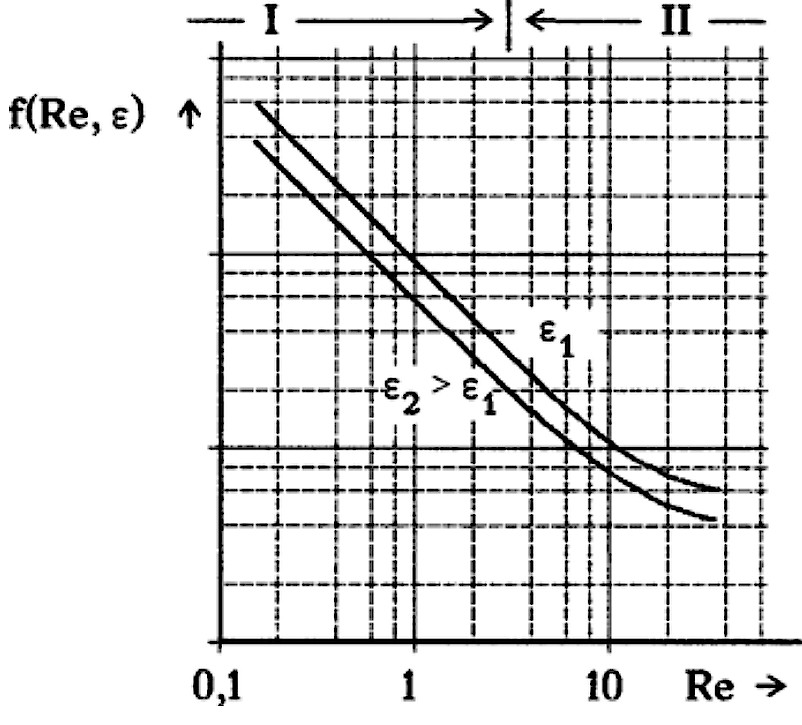
\includegraphics[width=0.4\textwidth]{Bilder/f_von_Re_epsilon.jpg}
\vspace{0em}
 \caption[]{Widerstandsfunktion für die Durchströmung von Schüttgütern, gemäß \cite[S. 146]{Stiess2008}}\label{fig:schuettungsdurchströmung}
\end{figure}

Die Widerstandsfunktion kann gemäß folgender Gleichung berechnet werden: \vspace{-0.3em}

\begin{equation}
\label{eq:widerstandsf_re}
f(\mathrm{Re}_x,\varepsilon)=\frac{\mathrm{Konstante}\,(\varepsilon)}{\mathrm{Re}_x}
\end{equation}

\vspace{0.3em} Die \glqq Konstante\grqq{}, zur Berechnung der Widerstandsfunktion, muss von der Porösität der Schüttung abhängen. Gemäß Abbildung \ref{fig:schuettungsdurchströmung} ist der Grenzwert, zwischen denen die Strömung unterschieden wird, eine Reynoldszahl des Betrags von ca. 3.\\

Die Darcygleichung ist für die Berechnung von strömungsinduzierten Druckverlusten $\Delta p$, zäh durchströmter Schüttungen (I) anwendbar. Unter der Annahme, dass das \mbox{$\Pi$-Theorem} mit den Lösungen $\bigl($Gleichung ($\ref{eq:eulerpi}-\ref{eq:porösität}$)$\bigr)$ nach der Eulerzahl auflösbar ist, das Schüttungen \textit{homogen} sind und \textit{Isotropie} innerhalb der Schüttung vorliegt, gilt Gleichung \cite[S. 145]{Stiess2008}: 

\begin{equation}
\label{eq:euler_pi}
Eu = \frac{\Delta L}{d} \cdot f(\mathrm{Re}_x,\varepsilon)
\end{equation}

\vspace{0.5em} Werden die Gleichungen (\ref{eq:widerstandsf_re}) und (\ref{eq:partikel_re}) in die Eulergleichung (\ref{eq:euler_pi}) engesetzt, erhält man \vspace{0.5em}

\begin{equation}
\label{eq:druck_laenge_darcy}
\frac{\Delta p}{\Delta L} = \frac{\mathrm{Konstante} \, (\varepsilon)}{\bar{x}^2} \cdot 	\eta \cdot \bar{v} .
\end{equation}

\vspace{0.5em} Die Schichteigenschaften werden in der Durchlässigkeit $B$ wie folgt zusammengefasst: \vspace{0.5em}

\begin{equation}
\label{eq:B}
B \equiv \frac{\bar{x}^2}{\mathrm{Konstante}\,(\varepsilon)}
\end{equation}

\vspace{0.3em} Die Durchlässigkeit $B$ muss für jede Schüttung empirisch ermittelt werden und wird in [$m^2$] angegeben. Die Durchlässigkeit charakterisiert die Porenquerschnitte \cite[S. 147]{Stiess2008}. Dadurch vereinfacht sich Gleichung (\ref{eq:druck_laenge_darcy}) zu folgender Gleichung: \vspace{0.5em}

\begin{equation}
\label{eq:druck_laenge_darcy_B}
\frac{\Delta p}{\Delta L} = \frac{\eta \cdot \bar{v} }{B}
\end{equation}


\newpage
\subsubsection{Ableitung der Filtergleichung aus der Darcygleichung}

Um eine Filtergleichung für den Betriebszustand einer konstanten, irreversiblen Druckdifferenz $\Delta p_{\mathrm{irr}}$ zu erhalten, muss die Ableitung gemäß \cite[S.100 ff.]{Stiess2013_verfahrensmechanik_band2} mit folgenden Annahmen erfolgen:


\begin{enumerate}
\item Die Massenkonzentration $c_\mathrm{m}$ bzw. die Volumenkonzentration $c_{\mathrm{vs}}$ der Suspension  bleibt zeitlich und örtlich Konstant,
\item Das gewonnene Filtrat ist Feststofffrei,
\item Der FIlterkuchen weist eine homogene Isotrope Struktur auf,
\item Filterkuchen sowie Filtermittel werden zäh Durchströmt (I).
\end{enumerate}

Das folgende mathematische Modell, zur Ableitung der Filtergleichung, liegt der Abbildung \ref{fig:filtergleichungsmodell} zugrunde.

\begin{figure}[h!] %[htbp!] 
\begin{center}
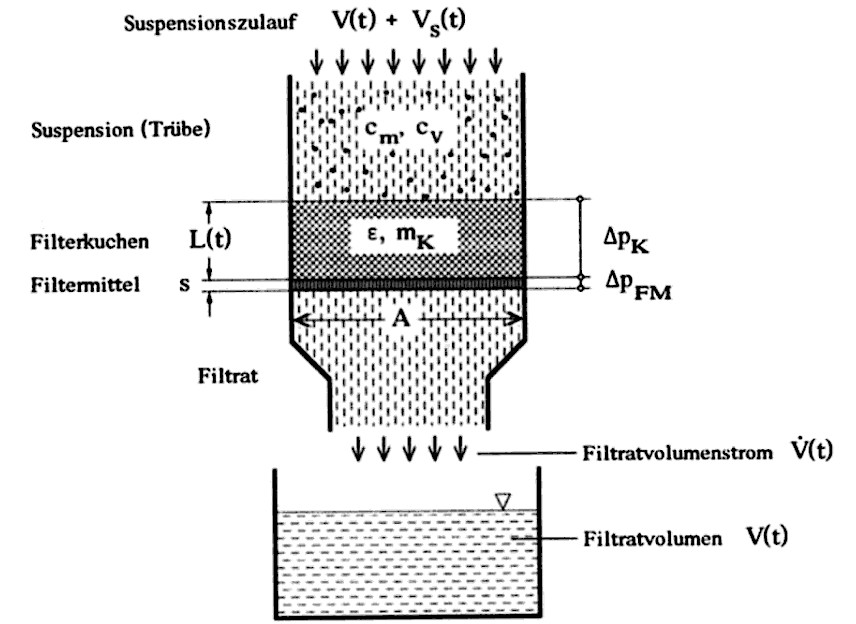
\includegraphics[width=0.7\textwidth]{Bilder/HAW/filterkuchenmodell.jpg}
\end{center}
\vspace{0em}
 \caption[Filterkuchenmodell zur Ableitung der Filtergleichung]{Filterkuchenmodell zur Ableitung der Filtergleichung, gemäß \cite[S.100 ff.]{Stiess2013_verfahrensmechanik_band2}}\label{fig:filtergleichungsmodell}
\end{figure}


Der gesamte irreversible (irr.) Druckverlust $\Delta p_{\mathrm{irr}}$ ist eine Summe aus filterkucheninduziertem $\Delta p_{\mathrm{K}}$ und filtermittelinduziertem  $\Delta p_{\mathrm{FM}}$ Druckverlust.

\begin{equation}
\label{eq:irr_druckverlust}
\Delta p_{\mathrm{irr}} = \Delta p_{\mathrm{K}} + \Delta p_{\mathrm{FM}}
\end{equation}

Der Druckverlust des Filtermittels, mit der Filtermitteldicke $s$ und der Filtermitteldurchlässigkeit $B_{\mathrm{FM}}$, kann gemäß Gleichung (\ref{eq:druck_laenge_darcy_B}) wie folgt berechnet werden:

\begin{equation}
\label{eq:filtermitteldpdt}
\Delta p_{\mathrm{FM}} = \frac{\eta  \cdot s}{B_{\mathrm{FM}}}  \cdot  \frac{\dot{V}}{A}
\end{equation}

\vspace{0.4em} Der Volumenstrom ist im Verlauf der Filtration zeitlich nicht konstant, daher ist das Volumen $V$ über die Zeit zu differenzieren: \vspace{-0.1em}

\begin{equation}
\label{eq:filtermitteldpdt}
\Delta p_{\mathrm{FM}}(t) = \frac{\eta   \cdot s}{B_{\mathrm{FM}} \cdot A}  \cdot  \frac{ \mathrm{d}\, V}{\mathrm{d}\, t}
\end{equation}

\vspace{0.6em} Analog ist zur Berechnung des Druckverlustes durch den Filterkuchen, mit der zeitlich anwachsende Filterkuchendicke  $L(t)$ und dessen Durchlässigkeitskonstante $B_{\mathrm{FM}}$ (unter der Annahme von \textit{Isotropie} und \textit{Homogenität}), folgender Ansatz zu wählen: \vspace{-0.1em}

\begin{equation}
\label{eq:filterkuchendpdt}
\Delta p_{K}(t) = \frac{\eta   \cdot L(t)}{B_{\mathrm{K}} \cdot A}  \cdot  \frac{ \mathrm{d}\, V}{\mathrm{d}\, t}
\end{equation}

\vspace{0.4em} Summiert man Gleichung (\ref{eq:filtermitteldpdt}) und Gleichung (\ref{eq:filterkuchendpdt}) erhält man Gleichung (\ref{eq:irr_druckverlust_dpdt}).

\begin{equation}
\label{eq:irr_druckverlust_dpdt}
\Delta p_{\mathrm{irr}}(t) =  \frac{\eta}{A} \cdot \Biggl[ \frac{L(t)}{B_\mathrm{K}}+\frac{s}{B_{\mathrm{FM}}} \Biggr] \cdot  \frac{ \mathrm{d}\, V}{\mathrm{d}\, t}
\end{equation}

\vspace{0.6em} Durch die Einführung des Filtermittelwiderstandes $\beta=s/B_{\mathrm{FM}}$ und des spezifischen Filterkuchenwiderstands $\alpha_\mathrm{V}= 1/B_\mathrm{K}$ vereinfacht sich Gleichung (\ref{eq:irr_druckverlust_dpdt}) zu: \vspace{0.1em}

\begin{equation}
\label{eq:irr_alpha_beta_dpdt}
\Delta p_{\mathrm{irr}}(t) =  \frac{\eta}{A} \cdot \Bigl[ \alpha_\mathrm{V} \cdot L(t) + \beta \Bigr] \cdot  \frac{ \mathrm{d}\, V}{\mathrm{d}\, t}
\end{equation}

\vspace{0.6em} Unter der Voraussetzung (1) sowie (3), dass das Kuchenvolumen $V_\mathrm{K}$ und das Filtratvolumen $V$ in einer direkt proportionalen Beziehung zueinander stehen ($V_\mathrm{K} \sim V$), kann die Proportionalitätskonstante $\kappa$ eingeführt werden.
\vspace{0.1em}

\begin{equation}
\label{eq:kappa}
L(t)=\frac{V_\mathrm{K}(t)}{A}=\kappa \cdot \frac{V(t)}{A}
\end{equation}

\vspace{0.4em} Ein weiterer Vorteil der Einführung der Proportionalitätskonstante $\kappa$, ist die Substitution der schwierig zu messenden Filterkuchendicke $L(t)$, durch das Filtratvolumen $V(t)$, die sich präzise bestimmen lässt. Setzt man Gleichung (\ref{eq:kappa}) in Gleichung (\ref{eq:irr_alpha_beta_dpdt}) ein, dann erhält man eine leicht auswertbare Gleichung folgender Form:

\begin{equation}
\label{eq:irr_alpha_beta_kappa_dpdt}
\Delta p_{\mathrm{irr}}(t) =  \frac{\eta}{A} \cdot \Bigl[ \frac{\alpha_V \cdot \kappa}{A} \cdot V(t) + \beta \Bigr] \cdot  \frac{ \mathrm{d}\, V}{\mathrm{d}\, t}
\end{equation}



\vspace{2em} 

\subsubsection{Ableitung der Filtergleichung für die Betriebsweise mit einer konstanten Druckdifferenz}

Filtrationen kann man durch unterschiedliche Betriebsweisen realisieren. In der folgenden Auflistung sind die möglichen Varianten aufgelistet:

\begin{enumerate}[label=\Roman*]
\item \quad Isobar -- $\Delta p = \mathrm{konstant}$,
\item \quad Isochor -- $\Delta V = \mathrm{konstant}$,
\item \quad Polytrop --  $\Delta p$ und $\Delta V$ variabel.
\end{enumerate}

Für die isobare Filtration, mit einer konstanten Druckdifferenz $\Delta p_{\mathrm{konst,irr}}$ gilt der nun folgende Ansatz.

\vspace{0.4em} Durch Trennung der Variablen der Gleichung (\ref{eq:irr_alpha_beta_kappa_dpdt}), erhält man Gleichung (\ref{eq:irr_alpha_beta_kappa_trennung_dpdt}) wodurch man durch Integration Gleichung (\ref{eq:irr_alpha_beta_kappa_integration_dpdt}) erhält.

\begin{align}
\mathrm{d}\,t &=  \frac{1}{\Delta p_{\mathrm{konst,irr}}} \cdot \Bigl[ \frac{\eta \cdot \alpha_\mathrm{V} \cdot \kappa}{A^2} \cdot V(t) + \frac{\beta \cdot \eta}{A} \Bigr] \cdot \mathrm{d}\, V \label{eq:irr_alpha_beta_kappa_trennung_dpdt}\\[1.2em]
t &= \frac{\eta \cdot\alpha_\mathrm{V} \cdot \kappa}{A^2 \cdot 2 \cdot \Delta p_{\mathrm{konst,irr}}} \cdot V^2(t) + \frac{\eta \cdot \beta}{A \cdot \Delta p_{\mathrm{konst,irr}}} \cdot V(t) \label{eq:irr_alpha_beta_kappa_integration_dpdt}
\end{align}

\vspace{0.4em}Löst man Gleichung \ref{eq:irr_alpha_beta_kappa_integration_dpdt} nach $V(t)$ auf, erhält man Gleichung (\ref{eq:filtergleichung_V}), wodurch die zeitlich zunehmende Filtratmenge berechnet wird. Die grafische Darstellung einer Filterkurve ist der Abbildung \ref{fig:filterkurve} zu entnehmen.

\begin{equation}
\label{eq:filtergleichung_V}
V(t)= \sqrt{
\Bigl( \frac{\beta \cdot A}{\alpha_V \cdot \kappa} \Bigr)^2
+ \frac{2 \cdot A^2 \cdot \Delta p_{\mathrm{konst,irr}}}{\eta \cdot \alpha_\mathrm{V} \cdot \kappa} \cdot t
} -\frac{\beta \cdot A}{\alpha_\mathrm{V} \cdot \kappa}
\end{equation}


\begin{figure}[h!] %[htbp!] 
\centering
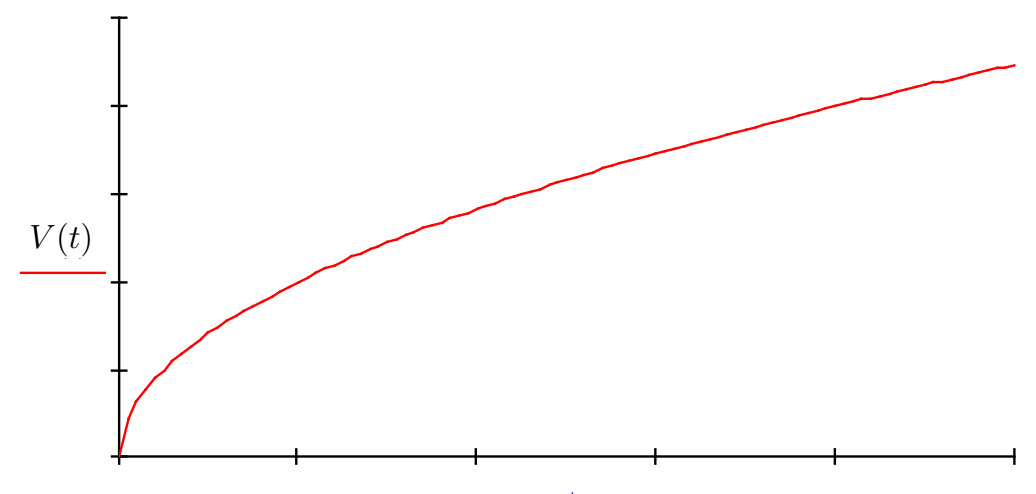
\includegraphics[width=0.7\textwidth]{Bilder/Filterkurve.jpg}
\vspace{0em}
 \caption[]{Filterkurve bei isobarer Betriebsweise \cite[S. 8]{Kuchenfiltration_Geweke2020}}\label{fig:filterkurve}
\end{figure}


Eine weitere Lösung ist die Linearisierung der Gleichung \ref{eq:irr_alpha_beta_kappa_integration_dpdt}, durch Division durch das Volumen als Funktion der Zeit $V(t)$. Die grafische Darstellung der Gleichung (\ref{eq:irr_alpha_beta_kappa_integration_linearisiert_dpdt}) ist der Abbildung \ref{fig:filtergerade_isobarebetriebsweise} zu entnehmen.

\begin{equation}
\label{eq:irr_alpha_beta_kappa_integration_linearisiert_dpdt}
\frac{t}{V(t)} = \underbrace{\frac{\eta \cdot\alpha_\mathrm{V} \cdot \kappa}{A^2 \cdot 2 \cdot \Delta p_{\mathrm{konst,irr}}}
\cdot V(t)}_{\substack{a_1}}  +  \underbrace{\frac{\eta \cdot \beta}{A \cdot \Delta p_{\mathrm{konst,irr}}}}_{\substack{a_0}}
\end{equation}

\begin{figure}[h!] %[htbp!] 
\centering
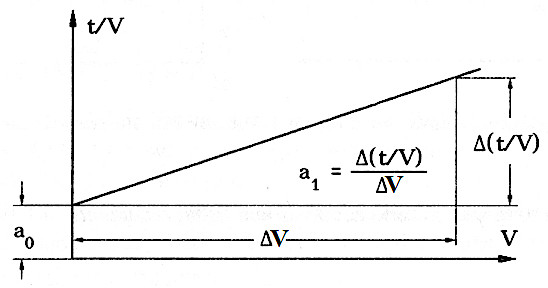
\includegraphics[width=0.7\textwidth]{Bilder/filtergerade.jpg}
\vspace{0em}
 \caption[Filtergerade für die isobare Betriebsweise]{Filtergerade für die isobare Betriebsweise \cite[S.102 ff.]{Stiess2013_verfahrensmechanik_band2}}\label{fig:filtergerade_isobarebetriebsweise}
\end{figure}

%\vspace{0.2em} 

\newpage
Die Ableitungen der Darcy-Gleichung für die isochore (II) oder polytrope (III) Betriebsweise werden im Rahmen dieser Arbeit nicht erläutert.




\paragraph*{Anmerkung}

Neben der Darcy-Gleichung existieren noch weitere empirische Gleichungen, zur Beschreibung von Schüttungen. Die, neben der Darcy-Gleichung, häufig genutzten empirischen Gleichungen werden nachfolgend aufgelistet \cite[S. 148 ff.]{Stiess2008}\cite[S. 1426 f.]{vdiwaermeatlas2019}:

\begin{itemize}
	\item zäh durchströmte Schüttung
	\begin{itemize}
		\item Carman-Kozeny-Gleichung (höherer Detailgrad)
	\end{itemize}
	\item zäh \textit{turbulent} durchströmte Schüttung 
	\begin{itemize}
		\item Ergun-Gleichung
		\item Brauer-Gleichung
	\end{itemize}
\end{itemize}

Das Model der Einzelpartikelumströmung nach \textit{Molerus} kann bspw. dem VDI-Wärmeatlas entnommen werden \cite[S. 1427 ff.]{vdiwaermeatlas2019}.



\newpage
\subsection{Verfahrenstechnischer Prozess: Gas-Feststoff Wirbelschicht}

Das Wirbelschichtverfahren ist eine verfahrenstechnische Grundoperation (\textit{engl. Unit Operation}). Dieses Verfahren wird im Sprachgebrauch der Wirbelschichttechnik auch Fluidisierung (\textit{engl. fluidization}) genannt. Die Fluidisierung wird für verschiedene Zwecke eingesetzt, wie z.B. zum Fördern, Mischen, Agglomerieren \cite{Ding2010}, Trocknen, Rösten, aber auch in der Reaktortechnik, wie zum Verbrennen von Schüttgütern \cite{Reuter2011}. Das Partikelbett (\textit{engl. fixed-bed}) liegt in einem Wirbelschichtapparat auf Anströmböden $A_\mathrm{a}$. Im Labormaßstab entspricht das einem Filtergewebe.

\subsubsection{Festbett-/Wirbelschichtparameter}

Ein Schüttgutpartikelbett, welches keine Anströmung durch ein Fluid erfährt oder keinen fluidähnliches Verhalten hat, wird als Festbett (\textit{engl. fixed-bed}) bezeichnet. Es kennzeichnet sich durch folgende Parameter aus \cite[S. 1561 ff.]{vdiwaermeatlas2019}:

\begin{itemize}
\item das Schüttguttvolumen $V_{\mathrm{fb}}$ 
\item der Masse $m_{\mathrm{fs}}$ 
\item die Dichte der Partikel $\rho_{\mathrm{fs}}$  
\item der Festbettporösität $\varepsilon_{\mathrm{fb}}$, der Partikelgrößenverteilung; die dem Feinheitsmerkmal der Partikel, dem sog. Sauterdurchmesser $d_{32}$ ($d_{32}=6/S_\mathrm{V}$) inhärent ist
\item und der apparatabhängigen Anströmfläche $A_\mathrm{a}$ 
\item Die mittlere Leerrohrgeschwindigkeit $\bar{v}$ 
\end{itemize}

In der Wirbelschichttechnik verwendet man die \textbf{Leerrohrgeschwindigkeit}. Die Leerrohrgeschwindigkeit $\bar{v}$ ist auf die leere Wirbelschichtquerschnittsfläche $A_\mathrm{a}$ bezogene Fluidgeschwindigkeit. 

Des Weiteren werden für die vollständige Berechnung der Wirbelschicht weitere dimensionslose Kennzahlen benötigt, auf die im Rahmen dieser Arbeit nicht weiter eingegangen wird. Nähere Informationen können bspw. dem VDI-Wärmeatlas entnommen werden \cite[S. 1561 ff.]{vdiwaermeatlas2019}.

\subsubsection{Klassifizierung von Schüttgütern nach Geldart}

Nicht alle Schüttgüter sind für Wirbelschichten gleichermaßen geeignet. Geldart hat eine Klassifizierung durchgeführt (siehe Abbildung \ref{fig:geldart}). Im sog. Geldart-Diagramm ist auf der Ordinate die Dichtedifferenz zwischen Fluid und Partikel dargestellt. Auf der Abzisse ist der mittlere Partikeldurchmesser $\bar{d}_{32}$ (gemäß Grafik $d_\mathrm{p}$) aufgetragen. In der Abbildungen sind vier Cluster (C, A, B, D), zwei breite und ein schmaler Übergangsbereich zu erkennen. Das Verhalten der Schüttgüttypen in einer Wirbelschicht unterscheidet sich z.T. signifikant \cite[S. 1566]{vdiwaermeatlas2019}.

\paragraph{Gruppe C} Schüttgüter die nach Klasse C klassifiziert werden, haben kleine mittlere Partikeldurchmesser und weisen größere Haftkräfte auf, als die durch die Strömung induzierte Kraft. Es bilden sich Kanäle aus. Eine Ausbildung einer Wirbelschicht ist nur durch apparative Hilfsmittel oder der Zusatz durch Fließmittel möglich \cite[S. 1566]{vdiwaermeatlas2019}.

\paragraph{Gruppe A} Oberhalb der Lockerungsgeschwindigkeit bildet sich eine homogene WIrbelschicht aus. Wird die Leerrohrgeschwindigkeit weiter erhöht Bilden sich Blasen aus, die sich beim emporsteigen zusammenschließen (Koaleszenz). Die Blasenaufstiegsgeschwindigkeit ist höher als die des Zwischenraumgas und die Blasengröße ist ab erreichen einer bestimmten Betthöhe begrenzt. Wird die Anströmung unterbrochen, kollabiert das Partikelbett langsam \cite[S. 1566]{vdiwaermeatlas2019}. 

\paragraph{Gruppe B}
Unmittelbar nach Überschreiten der Lockerungsgeschwindigkeit bilden sich Blasen aus.  Die Blasenaufstiegsgeschwindigkeit ist höher als die des Zwischenraumgas. Die Blasengröße ist nicht begrenzt. Die Bettausdehnung ist geringer als die der Schüttgüter der Gruppe A. Wird die Anströmung unterbrochen kollabiert das Bett schlagartig \cite[S. 1566]{vdiwaermeatlas2019}. 

\paragraph{Gruppe D}
Die Partikel dieser Gruppe sind groß und weisen eine große Dichte auf. Die Blasen haben eine geringere Aufstiegsgeschwindigkeiten als die des Zwischenraumgases. Nutzt man keinen breiten Anströmboden sondern nur eine Zentrale Bohrung, dann bildet sich bei hinreichend großer Anströmgeschwindigkeit eine Strahlschicht aus \cite[S. 1566]{vdiwaermeatlas2019}.  

\begin{figure}[h!] %[htbp!] 
\centering
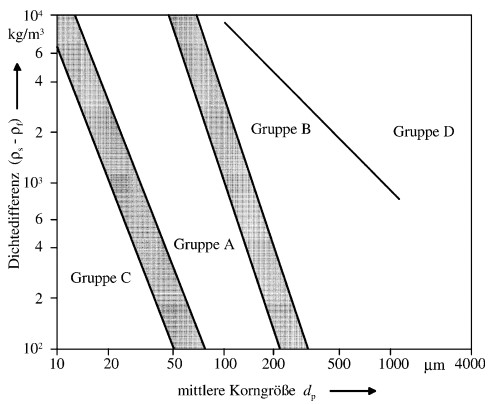
\includegraphics[width=0.6\textwidth]{Bilder/Geldart.jpg}
\vspace{0em}
 \caption[Klassifizierung von Schüttgütern nach Geldart]
 {Klassifizierung von Schüttgütern nach Geldart \cite[S. 1566 ff.]{vdiwaermeatlas2019}}\label{fig:geldart}
\end{figure}


 \pagebreak

 
\subsubsection{Wirbelschichtzustände eines für die Fluidisierung optimalen Schüttguts}

Um die Funktionsweise der Wirbelschicht zu verstehen, werden vier Zustände der Wirbelschicht; anhand eines für die sog. \textit{Fluidisierung} optimalen Schüttguts (Klassifizierung nach Geldart A), gemäß der Abbildung  \ref{fig:wirbelschichtzustände}; beschrieben. In der Abbildung \ref{fig:wirbelschichtzustände} sind Wirbelschichtzustände als Funktion der Anströmgeschwindigkeit schematisch dargestellt \cite[S. 1561 f.]{vdiwaermeatlas2019}.\\

\textbf{Abbildung \ref{fig:wirbelschichtzustände}\texttt{a}} zeigt ein Schüttgutfestbett, welches mit einem $\dot{V}$ Volumenstrom beaufschlagt wird, welcher kleiner ist als der minimale Fluidisiervolumenstrom $\dot{V}_{\mathrm{mf}}$. Die Mehrheit der Partikel befindet sich in Kontakt.\\

Sobald die Anströmgeschwindigkeit der minimalen Fluidisiergeschwindigkeit entspricht, ist der sog. Lockerungspunkt erreicht (\textbf{Abbildung \ref{fig:wirbelschichtzustände}\texttt{b}}). Das Schüttgut nimmt fluidähnliches Verhalten an. Das gesamte, nun Fluidbettbett ist in einer homogenen Bewegung. Es liegt der Zustand der Minimalfluidisation vor.\\


\begin{figure}[t!] %[htbp!] 
\centering
\includegraphics[width=0.85\textwidth]{Bilder/wirbelschichtzustände.jpg}
\vspace{0em}
 \caption[Wirbelschichtzustände als Funktion der Anströmgeschwindigkeit]
 {Wirbelschichtzustände als Funktion der Anströmgeschwindigkeit \cite[S. 1562]{vdiwaermeatlas2019} }\label{fig:wirbelschichtzustände}
\end{figure}



Wird die Strömungsgeschwindigkeit weiter erhöht tritt eine Blasenbildung auf. Welche Form der Blasenbildung entsteht ist unter anderem abhängig von der Geometrie des Apparates (vgl. \textbf{Abbildungen \ref{fig:wirbelschichtzustände}\texttt{c}} und \textbf{\ref{fig:wirbelschichtzustände}\texttt{d}}). Beim Aufsteigen der vereinzelten Gasblasen verschmelzen diese. Dieser Vorgang wird Koaleszenz genannt.\\

Ist die Anströmgeschwindigkeit viel größer als die minimale Fluidisiergeschwindigkeit und erreicht bzw. übersteigt die Sinkgeschwindigkeit der Partikel (Einzelkornsinkgeschwindigkeit), dann bricht die Blasenbildung auf und der Feststoff wird ausgetragen (siehe \textbf{Abbildung \ref{fig:wirbelschichtzustände}\texttt{e}}). Wie in der \textbf{Abbildung} \ref{fig:wirbelschichtzustände}\texttt{e} zu erkennen, bilden sich Feststoffsträhnen, dadurch ist die Aufrechterhaltung der Wirbelschicht möglich. Wenn das Ziel der Wirbelschicht nicht der Partikelförderung entspricht, dann ist eine Rückführung der Partikel, bspw. durch einen nachgeschalteten Zyklon, gemäß \textbf{Abbildung} \ref{fig:wirbelschichtzustände}\texttt{e} zu realisieren.\\

\paragraph{Anmerkung}
Schüttgüter der Geldartklassifizierung C und D benötigen andere apparative Lösungen. Es wird auf Fachliteratur wie bspw. den VDI-Wärmeatlas hingewiesen.\\


\subsubsection{Druckverlust beim Betrieb einer Wirbelschicht}

Die Wirbelschicht wird dadurch ausgezeichnet, dass sich das Partikelbett in einem definierten Volumenstromintervall wie ein Fluid verhält. Das Partikelbett hat in dem Intervall zwischen der \textbf{Lockerungsgeschwindigkeit} $\bar{v}_{\mathrm{mf}}$ und der Partikelaustragsgeschwindigkeit fluidähnliche Eigenschaften. Die Partikelaustragsgeschwindigkeit kann mit der \textbf{Einzelkornsinkgeschwindigkeit} $\bar{w}_{\mathrm{fs}}$ abgeschätzt werden. Das Leerrohrgeschwindigkeitsintervall der Fluidisierung ist somit  $[\bar{v}_{\mathrm{mf}};\bar{v}_{\mathrm{fs}}]$ \cite[S. 1562 ff.]{vdiwaermeatlas2019}. \\

\begin{figure}[b!] %[htbp!] 
\centering
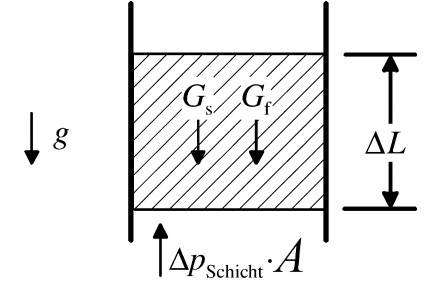
\includegraphics[width=0.5\textwidth]{Bilder/wirbelschicht_kraefte.jpg}
\vspace{0em}
 \caption[]{Wirbelschichtkräfftegleichgewicht an einem Wirbelschichtelement der Länge $\Delta L$ und Anströmfläche $A$, angelehnt an \cite[S. 1562]{vdiwaermeatlas2019}}\label{fig:wirbelschicht_kraefte}
\end{figure}

Der Wirbelschicht liegt ein Kräftegleichgewicht zugrunde. Im stationären Zustand befinden sich die Partikel in der Schwebe. In der Abbildung \ref{fig:wirbelschicht_kraefte} ist das Kräftegleichgewicht eines Wirbelschichtelements skizziert. Das Kräftegleichgewicht eines Wirbelschichtelements der Länge $\Delta L$ und der Anströmfläche $A_\mathrm{a}$ lässt sich wie folgt berechnen.

\begin{equation}
\label{eq:kraefte_ggw_ws}
\Delta P_{\mathrm{Schicht}} \cdot A_\mathrm{a} = G_{\mathrm{fs}} + G_{\mathrm{f}}
\end{equation}

Das Feststoffgewicht $G_{\mathrm{fs}}$ ergibt sich für eine Schicht mit der Feststoffdichte $\rho_{\mathrm{fs}}$ durch

 \begin{equation}
 \label{eq:feststoffgewicht}
G_{\mathrm{fs}}=\rho_{\mathrm{fs}}~(1-\varepsilon)~g~A_{\mathrm{a}}~\Delta L
 \end{equation}

und das Gewicht des Fluids, mit der Fluiddichte $\rho_\mathrm{f}$ durch 

 \begin{equation}
  \label{eq:fluidgewicht}
G_{\mathrm{f}}=\rho_{\mathrm{f}}~\varepsilon~g~A_{\mathrm{a}}~\Delta L.
 \end{equation}
 
Der Druckabfall einer Schicht berechnet sich mit den Gleichungen \ref{eq:feststoffgewicht} und  \ref{eq:fluidgewicht} aus Gleichung \ref{eq:kraefte_ggw_ws} wie folgt:
 
\begin{equation}
\label{eq:druckabfall_schicht}
\Delta P_{\mathrm{Schicht}} = \underbrace{ (\rho_{\mathrm{fs}}-\rho_\mathrm{f})(1-\varepsilon)~g~\Delta L}_{\substack{=\Delta p_{\mathrm{irr}}}} +\underbrace{\rho_\mathrm{f}~g~\Delta L}_{\substack{=\Delta p_{\mathrm{reversibel}}}}
\end{equation}

\vspace{0.8em} Der erste Term repräsentiert den irreversiblen Anteil des Druckabfalls. Um die Partikel in der Schwebe zu halten wird Energie benötigt, die sich anhand des ersten Terms berechnen lässt. Der irreversible Anteil des Druckabfalls setzt sich aus der Gewichtskraft pro Fläche (Gleichung \ref{eq:feststoffgewichtskraft}), abzüglich der volumenstrominduzierten Auftriebskraft pro Fläche  (Gleichung \ref{eq:partikelauftriebskraft}) zusammen \cite[S. 1562 ff.]{vdiwaermeatlas2019}.

 \begin{align}
p_{\mathrm{fs}} &= \rho_{\mathrm{fs}}~(1-\varepsilon)~g~\Delta L \label{eq:feststoffgewichtskraft} \\
p_{\mathrm{f}} &= -\rho_{\mathrm{f}}~(1-\varepsilon)~g~\Delta L \label{eq:partikelauftriebskraft}
 \end{align}

Der zweite Term der Gleichung (\ref{eq:druckabfall_schicht}) repräsentiert die potentielle Energie des geförderten Fluids, der Höhe $\Delta L$. Diese \mbox{Energie} kann im Falle einer Flüssig-Feststoffwirbelschicht, bspw. durch die Nutzung einer Turbine, zurückgewonnen werden \cite[S. 1562 ff.]{vdiwaermeatlas2019}. \\

Die Leerrohrgeschwindigkeit der Minimalfluidisation $v_{\mathrm{mf}}$, auch Lockerungsgeschwindigkeit genannt, kann empirisch ermittelt werden. Wird der dimensionslose Druck gegen die Leerrohrgeschwindigkeit aufgetragen, ist die Lockerungsgeschwindigkeit mit dem erreichen des dimensionslosen Drucks mit dem Betrag von 1 erreicht (siehe Abbildung \ref{fig:lockerungsgeschwindigkeit}). Ab dem Überschreiten der Leerrohrgeschwindigkeit ist der Druckverlust, relativ zur Umgebung $\Delta p$ ebenfalls konstant, dazu wird eine doppelt logarithmische Auftragung empfohlen. Simultan zum Anstieg der Leerrohrgeschwindigkeit, ab der Lockerungsgeschwindigkeit $v_{\mathrm{mf}}$, ist eine Expansion der Wirbelschicht messbar. Die Druckkonstanz ab dem Lockerungspunkt ist damit zu erklären, dass die erhöhte Energiezufur für die Expansion der Wirbelschicht genutzt wird. Ab einer bestimmten Expansion schließen sich Hohlräume zusammen und es kommt zur Blassenbildung (siehe Abbildung \ref{fig:wirbelschichtzustände}). Dieser Effekt liegt der Koalesenz zugrunde.

\begin{figure}[t!] %[htbp!] 
\centering
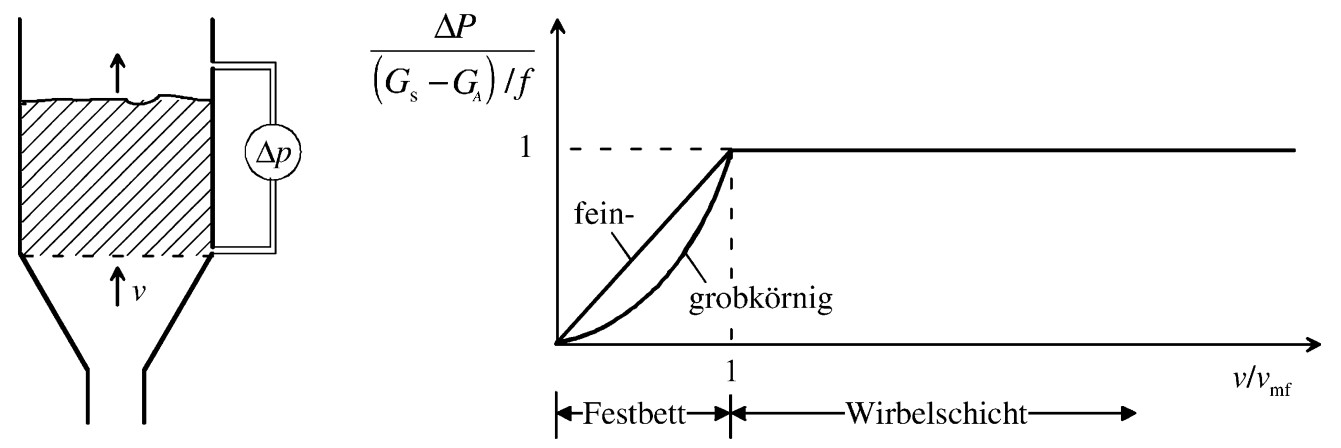
\includegraphics[width=1\textwidth]{Bilder/Lockerungspunkt.jpg}
\vspace{0em}
 \caption[Konstantz des dimensionslosen Drucks, ab dem überschreiten der Lockerungsgeschwindigkeit]{Konstantz des dimensionslosen Drucks, ab dem überschreiten der Lockerungsgeschwindigkeit $v_{\mathrm{mf}}$, in Anlehnung an  \cite[S. 1563]{vdiwaermeatlas2019}}\label{fig:lockerungsgeschwindigkeit}
\end{figure}

\subsubsection{Anmerkung}
 Für tiefgreifendes Wissen zur Berechnung von Wirbelschichten wird auf Fachliteratur, wie dem VDI Wärmeatlas \cite[S. 1561 ff.]{vdiwaermeatlas2019}, verwiesen.





\newpage
\subsection{Signalverarbeitung}

In diesem Abschnitt werden die Grundlagen der Signalverarbeitung erläutert. Im ersten Abschnitt werden nochmals die Grundlagen der Rechnerkommunikation erläutert, gefolgt von dem Unterschied zwischen analogen und digitalen Signalen. Es werden einige Kabelgebundene Schnittstellen, aber auch Schnittstellen die via Funk funktionieren, erläutert.\\


\subsubsection{Vom Bit bis zur \glqq vom Menschen lesbaren\grqq{} Alphanumeric}

Sobald man von digitalen Daten spricht, ist von Bit encodierten, binären Daten die Rede. PC's sind in der Lage, diese Form der Signale direkt zu verarbeiten. In der Abbildung \ref{binary_data_sizes} sind verschiedene Datengrößen binärer Daten aufgezeigt. In der Abbildung variiert die Spanne der Datengrößenlänge von einem Bit bis zu einem Wort bestehend aus 16-Bit. Binäre digitale Daten sind diskret. Ein Bit hat zwei mögliche Zustände, an oder aus, die durch die binären Werte 0 oder 1 sowie den booleschen Ausdrücken \,{\Menlo true} oder \,{\Menlo false} repräsentiert werden können. Die Anzahl, wie viele Bit ein Zeichen (\textit{engl. character}) repräsentiert, kann sich unterscheiden. Häufig wird ein Byte bestehend aus 7 oder 8-{\Menlo Bit} verwendet. In der Abbildung \ref{binary_data_sizes} ist eine ByteLänge von 8-{\Menlo Bit}, häufig auch Oktett genannt, dargestellt. Ein Byte, welches aus 8-Bit besteht, hat 256 mögliche Zustände. Die Hälfte eines (8-Bit) Byte wird\, Nibble genannt \cite[S. 3]{hughes2010real}. Sind Signale ASCII encodiert, beträgt die Byte Länge 7 Bit. Der ASCII Zeichensatz beinhaltet somit 128 (0 - 127) Zeichen. ASCII-Tabellen können alle Zeichen der 7-Bit ASCII Codierung sowie die Zuordnung der dezimalen und hexadezimalen Werte entnommen werden. \\

\bildp{h}{0.6}
{binary_data_sizes.png}
{0em}
{Binary data sizes }
{Binary Data Sizes \cite[S. 3]{hughes2010real} }
{binary_data_sizes}


\paragraph*{Hexadezimal} Zeichen können neben der binärer und der dezimalen Darstellung auch Hexadezimal dargestellt werden. Die Hexadezimale Skala geht von 0 bis 9 gefolgt von A bis F. Die Skala hat somit eine dezimale Ziffernlänge von 16. Ein Nibble kann somit durch eine hexadezimale Ziffer dargestellt werden.\\


\subsubsection{Analoge und digitale Signale}

Möchte man Signale verarbeiten, dann ist zwischen zwei Signaltypen zu unterscheiden. Die reale Welt lässt sich durch ein Kontinuum von Zuständen beschreiben. Elektrische Messgeräte erfassen diese Zustände und erzeugen bspw. eine Spannung. Bei einer kontinuierlichen Messung würden bei einer definierten Frequenz, Signale in Form von Spannung generiert werden. Als Beispiel werfen wir einen Blick auf das Messen einer Temperatur. Bei diesem Beispiel nehmen wir einmal an, dass wir einen Temperaturfühler verwenden, der eine Messgenauigkeit von \SI{0.0001}{\degreeCelsius} besitzt. Bei der Messung der Temperatur von Wasser könnte man eine Gleitkommazahl (floating point number oder kurz float) von \SI{19,2334}{\degreeCelsius} angezeigt bekommen. Bis zur zweiten Messung könnte ein Temperaturausgleich zwischen Umgebung und dem Wasser erfolgt sein, was zu einem anderen Temperaturmesswert von bspw. \SI{12,240}{\degreeCelsius} führen könnte. Analoge Signale sind ein Kontinuum von Signalen. \\

\noindent PC's sind in der Lage digitale Signale sequenziell zu verarbeiten. Ein digitales Signale repräsentiert ein physikalisches Signal, Strom oder Spannung. In der Abbildung \ref{analog_digital_data_input} sind typische Methoden abgebildet, wie Daten eines Messobjekts akquiriert und an einen PC übermittelt werden. Oben im Bild sind vier Schalter zu erkennen, die einen Stromkreis schließen können. Diese Form der Signalübertragung wird diskret genannt. Auf dem Bild sind alle Schalter geöffnet, daher wäre pro Leiter ein binär Wert von 0 zu erwarten. In der Mitte der Abbildung ist ein Bit-serieller Datenstrom, anhand der Rechteckfunktion und den binär Werten, zu erkennen. Im unteren Teil der Abbildung ist ein analoges Signal zu erkennen, welches mittels eines analog zu digital Wandlers die Signale in eines von einem PC interpretierbares Signal wandelt. Die umgewandelten Daten werden mittels paralleler Schnittstelle an einen PC sendet.  

\bild{0.65}
{analog_digital_data_input.png}
{0em}
{Digital and analog data inputs \cite{hughes2010real}}
{Digital and analog data inputs \cite{hughes2010real}}
{analog_digital_data_input}



\subsubsection{Schnittstellen}

Messgeräte verfügen über Schnittstellen, über die Daten- und Steuersignale an andere Komponenten oder einen Messgerätebus erfolgen. An einen Messgerätebus werden Messgeräte (Slaves) und Rechner (Master) angeschlossen. Die Datenübertragung ist entweder Bit- oder Byte-seriell. Der Anschluss eines Messgeräts an einen PC kann über zwei Methoden erfolgen. Messgeräte können über analog Signalausgänge verfügen. Diese Signale müssen in einem analog/digital Wandler in ein digitales Signal gewandelt werden. Das Messgerät kann einen integrierten analog/digital Wandler und digitale Schnittstelle verfügen, über die Signale direkt an einen PC gesendet werden können. Die zwei Methoden können der Abbildung \ref{anschluss} entnommen werden \cite[S. 479]{Busch2015}. Diese analogen Signale müssen mittels einer Messkarte in ein digitales Signal umgewandelt werden, die im Anschluss in einem PC in einer Software weiter verarbeitet werden können. Im folgendem werden zwei Kabelgebundene (USB, RS-232) und zwei Kabellose (Bluetooth und W-LAN) Schnittstellen erläutert.

\bild{1}
{signalverarbeitung_hardware.jpg}
{0em}
{Digitale Schnittstelle oder über Messkarte}
{Anschluss eines Messgerätes an den PC, angelehnt an \cite[S. 479]{Busch2015}) 	\\  \textbf{oben} mit Messkarte, \\ \textbf{unten} mit digitaler Schnittstelle}
{anschluss}

\subsubsection{Verbinder}
\label{sec:verbinder}

Um eine Kommunikation zwischen den Geräten zu ermöglichen, bedarf es physikalischer Schnittstellen. Im Laborumfeld werden die USB Schnittstelle und die DB-9 Schnittstelle besonders häufig angetroffen. In der Abbildung \ref{db9_male} ist ein männlicher DB-9 Stecker abgebildet.

\bild{.5}
{db9_male-female.jpg}
{0em}
{DB-9 pin and socket numbering}
{DB-9 pin and socket numbering \cite{db9-male-female}}
{db9_male}



\subsubsection{Bitserielle Datenübertragung}

Es gibt verschiedene Möglichkeiten Signale, bzw. Daten zu übertragen. Eine Möglichkeit ist die serielle Datenübertragung. Eine genauere Bezeichnung wäre\, Bit-serielle Datenübertragung, denn genau genommen gibt es eine Reihe von\, Bit-seriellen Datenübertragungssystemen, unter anderem jedoch auch die\, Byte-serielle Datenübertragung. \\

\bild{0.6}
{serielle_datenuebertragung.png}
{-0.5em}
{Synchronous serial data communication}
{Synchronous serial data communication \cite[S. 52]{hughes2010real}}
{seriallio}

Des Weiteren gibt es zwei Formen der seriellen Datenübertragung, die synchrone und die asynchrone Datenübertragung. In Abbildung \ref{seriallio} ist eine synchrone Datenübertragung dargestellt. An dem Ausgang \textit{Clock Out} ist zu erkennen, dass das Gerät A den Takt und somit die Austauschrate der Schnittstelle vorgibt.Daten sind nur zum Zeitpunkt der fallenden Flanke des Taktsignals valide. Es ist zu erkennen, dass der Takt stets die Mitte der Bit Position trifft, um mögliche Fehler vorzubeugen. Die \glqq reale\grqq{} Rechteckfunktion ist eine Superposition von Funktion verschiedener Frequenzen, was dazu führt, dass bei aufsteigender Flanke und beim fallen der Flanke ein Einschwingen der Funktion stattfindet, bis sich ein konstanter Wert einstellt (siehe Abbildung \ref{squarefunction}). In der Praxis wird eine asynchrone Bit-serielle Datenübertragung häufiger genutzt. Eine fehlerfreie Kommunikation soll die sogenannte Datenflußsteuerung (\textit{engl. flow control}) übernehmen. Bei asynchroner Datenübertragung existiert somit kein Taktsignal. Bei einer asynchroner Datenübertragung kann der Bit Datenstrom neben der \glqq gewünschten\grqq{} Infromationen, z.B. von einer Messung, noch Datenflußsignale enthalten. Datenflußsignale können physikalische Signale sein. Diese Form der Flußsteuerung nennt sich \textit{Hardware-Handshake}. Eine andere Möglichkeit der Datenflußsteuerung ist der sog. \textit{Software-Handshake}. Die Datenflußsignale sind {\Menlo Startbit}, {\Menlo Stopbit} und {\Menlo Paritätsbit}, die ein Zeichen (\textit{engl. Character}) von einem anderen Zeichen abgrenzt. Zeichen können Buchstaben, Zahlen, Vorzeichen etc. sein, die binär versendet werden (0 oder 1) und beispielsweise ASCII encodiert sind.

\bild{0.65}
{square_waves.png}
{0em}
{Ideal versus real square waves}
{Ideal versus real square waves \cite[S. 5]{hughes2010real}}
{squarefunction}


\subsubsection{RS-232}

Die RS-232 Schnittstelle wurde in den 1960 Jahren von der Electronic Industrial Alliance (EIA) standardisiert. Jedes zu übertragende Zeichen (Zahl, Buchstabe, Sonderzeichen) wird zwischen 5 und 9 Bit codiert, wobei 7 und 8 Bit am gebräuchlichsten sind. Die Trennung von benachbarten Zeichen werden mit \textit{Start-} und \textit{Stopbit} realisiert. Die Übertragungsrate kann zwischen 0,3 Bd und 115,2 kBd betragen. Die Entfernung, die erzielt werden kann, ist stark vom verwendetem Kabel und der Übertragungsgeschwindigkeit abhängig. Es sind Entfernungen bis zu einem Kilometer realisierbar. Die Übertragungsgeschwindigkeit wird Baudrate genannt. Ein Bd entspricht 1 Zeichen pro Sekunde. Ein \textit{Symbol/Character} kann aus einem oder mehreren Bits besteht. Die Übertragungsrate ist somit im Vergleich zu anderen Schnittstellen mit, im Normalfall von einem Bit pro Zeichen, der Übertragungsgeschwindigkeit von 0,3 bis 115,2 kbit/s verhältnismäßig gering, reicht aber für die meisten Messtechnischen Anwendungen aus. Für die Kommunikation mittels RS-232 benötigt man eine sog. Flusssteuerung (engl. \textit{flow control}). Der Sender und der Empfänger müssen sich gegenseitig mitteilen, ob sie sende- oder empfangsbereit sind, um Datenverluste zu vermeiden. Die Signale, die man dafür benötigt, werden~ {\Menlo Handshake-Signale}~genannt. Der {\Menlo Handshake} lässt sich mit physischen Signalen über Steuerleitungen ({\Menlo Hardware-Handshake}) oder über digitale Signale (\textit{Software-Handshake}) realisieren. Die Software-Handshake Signale werden über die TxD Signalleitungen versendet. Für den \textit{Software-Handshake} ist die XON/XOFF und für den \textit{Hardware Handshake} die Datenflußsteuerung mittels CTS/RTS eine gängige Methode \cite[S. 480 f.]{Busch2015}. \\

RS-232 beschreibt Spannungspegel und Timing zwischen der Datenübertragungseinrichtung (DÜE) und Datenendeinrichtung (DEE). Nicht Bestandteil des Standards ist das eigentliche Übertragungsprotokoll, wie die Signale kodiert sind (z.B. ASCII), Fehlererkennung usw.. Solche Parameter müssen zwischen der Datenübertragungseinrichtung und der Datenendeinrichtung ausgehandelt werden \cite{wasistrs232}.



Üblicherweise werden für die Übertragung 9-Polige D-Sub Kabel verwendet, aber RS-232 ist nicht an diese Kabel und Stecker Kombination gebunden. In der AbbildungAbbildung \ref{db9_male} sind alle Signale und die Definition der Signale der DB-9 Schnittstelle aufgelistet. Bei der Verwendung eines Software-Handshake sind nur 3 Signalleitungen notwendig, da die Steuersignale über die Datenleitungen gesendet wird. Für den Datentransfer mittels 9-Poligen D-Sub Kabel (siehe Abbildung \ref{db9_male}), sind somit lediglich die Pins 2 (RxD), 3 (TxD) und 5 (GND) notwendig. Bei der Verwendung eines Hardware-Handshakes werden die Datenleitungen über die Pins 7 (RTS) und 8 (CTS) notwendig \cite{db9}. RS-232 ist eine Volt-basierte Schnittstelle. Der logische Wert wahr ({\Menlo true}) ist dem negativen Volt-Level zugeordnet und der logische Wert falsch ({\Menlo false}) ist dem positiven Volt-Level zugeordnet. Die Spanne der Volt-Spannung ist in RS-232 von +/- 3 V bis +/- 25 V spezifiziert.

\subsubsection{RS-485}

RS-485 ist eine Weiterentwicklung des RS-232 Standards. RS-485 ist ein Bus System, welche bis zu 32 Datensender und Empfänger verbinden kann und wird in der Prozessmess- und Prozessleittechnik angewandt. Es sind Übertragungsgeschwindigkeiten von bis zu 35\,MBit/s mit der Verwendung eines 10 Meter Kabels und 100~KBit/s mit einer Kabellänge von 1200 Meter möglich. Die RS-485 Schnittstelle verfügt über 2 Signalkabel. Die Polarität der beiden Kabel ist gegensätzlich (vergleiche Abbildung \ref{RS-485}). Beide Leitungen können Signale in beide Richtungen senden, jedoch nicht zur gleichen Zeit. Der Signalabgriff ist somit differentiell. Das Signal wird somit nicht gegen Null gemessen, sondern zwischen den zwei Leitern gegensätzlicher Polarität. In Abbildung \ref{RS-485} ist eine 8-Bit asynchrone Datenübertragung via RS-485 zu erkennen. Am Anfang und dem Ende der 8-Bit befindet sich ein Start- und ein Stopbit \cite[S. 222 f.]{hughes2010real}.

\begin{figure}[h!]
\centering
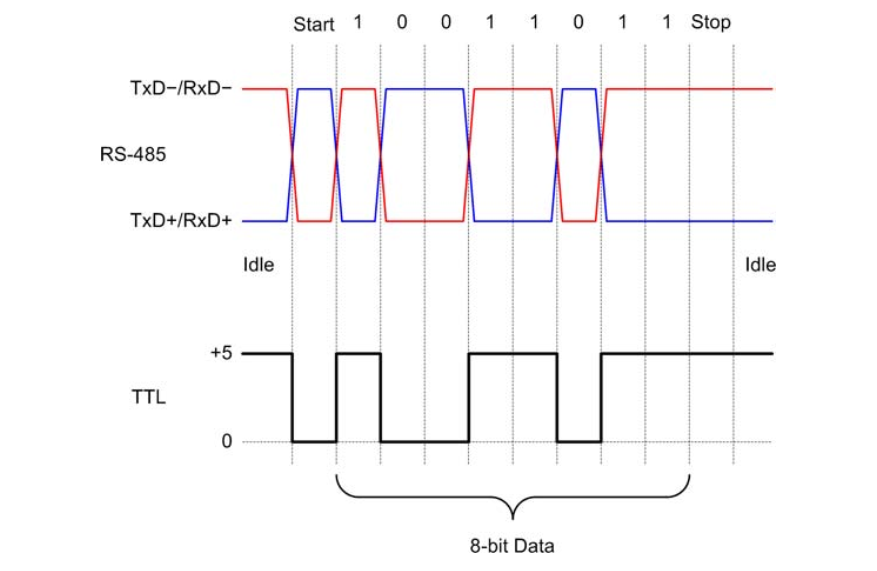
\includegraphics[width=0.7\textwidth]{Bilder/RS-485.png}
\caption{RS-485 signal levels \cite[S. 226]{hughes2010real}}
\label{RS-485} 
\end{figure}

%\bild{1}
%{RS-485.png}
%{0em}
%{RS-485 signal levels}
%{RS-485 signal levels \cite[S. 226]{hughes2010real}}
%{RS-485}

\subsubsection{USB}

Die überbrückbare Länge via USB liegt unter 5 m und liegt somit weit unter der Entfernung, die mit RS-232 möglich sind. USB wurde zwecks Schaffung einer einheitlichen Schnittstelle für alle Arten von PC's Laptops von INTEL entwickelt. USB-Kabel haben vier Leitungen, zwei für die \textit{Bit-serielle} bidirektionale Datenübertragung, eine Leitung für die +5V Versorgungsspannung und eine für das Massepotenzial. An einen USB-Anschluss eines PC's lassen sich theoretisch bis zu 128 Geräte anschließen, da die angeschlossenen Messgeräte durch den USB-Controller im PC mit einer 7-Bit-Adresse adressiert werden. Daraus folgen $2^7=128$ mögliche Messgeräte. Praktisch sind es 127, da die Adresse \glqq Null \grqq \, (000 0000) für die Geräte-Identifizierung genutzt wird. USB verfügt über zwei Eigenschaften, dem \glqq Hot-Plugging\grqq \, und dem \glqq Plug-and-Play\grqq . Dank dem Hot-Plugging ist es vor dem Verbinden eines Geräts mit dem PC nicht notwendig diesen auszuschalten. Dank Plug-and-Play konfiguriert sich die Verbindung selbst. USB 1.0 hat eine Übertragungsgeschwindigkeit von 1,5 bzw. 12 MBit/s, USB 2.0 bis zu 480 MBit/s und USB 3.0 hat eine Highspeedübertragungsrate von 5 GBit/s. Es ist je nach verwendetem Geräte möglich, diese an einer USB-Schnittstelle zu betreiben, die eine geringere Übertragungsrate besitzen als die USB-Schnittstelle des PC's.

\subsubsection{Bluetooth}
\label{sec:bluetooth}

Bluetooth ist eine kabellose Datenübertragungsmethode via Funk. Der Frequenzbereich ist zwischen 2,402 bis 2,480 GHz. Die Übertragungsdistanz beträgt ca. 10 m mit einer Übertragungsgeschwindigkeit von 2,1 MBit/s für die Spezifikation \textit{Bluetooth 2.0 + EDR} (Enhanced Data Rate) \cite[S. 481 f.]{Busch2015}.
Bluetooth 2.0 + EDR ist 2004 auf dem Markt erschienen. Bluetooth 4.2 Smart ist 2014 mit Einführungen von wichtigen Funktionen für das Internet der Dinge (IoT) erschienen. Bluetooth 5 (2017) ist die aktuellste Version und hat IoT im Fokus. Bluetooth 5 unterstützt Übertragungsraten von 2 MBit/s und einer Reichweite von maximal 250 m \cite{bt5}.\\

Drahtlose IoT- Lösungen nehmen in der produzierenden Industrie an Bedeutung zu. Da kabellose Netzwerke beim Aufbau von neuen Fertigungslinien flexibler sind als kabelgebundene Netzwerke, ist Bluetooth im Rahmen von Industrie 4.0 eine bedeutende Schnittstelle. Bluetooth Mesh Networking wurde unter anderem für industrielle drahtlose Sensornetzwerke konzipiert (WSN). Mit diesem Standard ist es möglich viele Geräte und Sensoren in einem Bluetoothnetzwerk kommunizieren zu lassen. Jedes Gerät wird \glqq Knoten\grqq \, genannt \cite{bti40}.

\paragraph*{Sicherheit: Mesh-Vernetzung per Bluetooth \cite{bti40}}

Die Netzwerksicherheit bei produzierenden Betrieben ist nicht verhandelbar. Die Sicherheit bei der Verwendung von Bluetooth, soll durch die sog. Mesh-Vernetzung gewährleistet werden. Die Informationssicherheit soll durch ein Schichtenmodell erreicht weden, dass auf voneinander getrennten Sicherheitsschlüssel basiert:

\paragraph*{Netzwerkschlüssel (NetKeys)} gelten für alle Nachrichten im Netzwerk, damit die Knoten sicher miteinander kommunizieren.

\paragraph*{Anwendungsschlüssel (AppKeys)} schützen Nachrichten zu bestimmten Anwendungen wie Klimaanlage, Beleuchtung oder physische Sicherheit.

\paragraph*{Geräteschlüssel (DevKey)} ermöglichen das Einrichten und Konfigurieren eines Knotens, um neue Geräte zum Netzwerk hinzuzufügen.

\subsubsection*{WLAN}

WLAN ermöglicht die Datenübertragung via Funk, ermöglicht jedoch eine signifikant höhere Übertragungsgeschwindigkeit und Übertagungsreichweite als Bluetooth. Mit der technischen Lösung 802.11 ist eine Gruppe von Standards für Funknetzwerke des Institute of Electrical and Electronics Engineers (IEEE) entwickelt worden. 

\subsubsection{Verarbeitung digitaler Signale in Labview}

Jeff Kodosky et al. hat in Zusammenarbeit mit der University of Texas die Programmiersprache G und die dazugehörige Enwicklungsumgebung LabVIEW entwickelt. 

LabVIEW stellt zum umsetzen spezieller Anwendung spezifische Werkzeuge und Modelle bereit. Das Ziel war es ein Tool zu entwickeln, wodurch Menschen mit unterschiedlichem know-how im Programmieren befähigt werden maßgeschneiderte Programme grafisch generieren zu können, da sich im Laborumfeld Versuchsaufbauten und somit auch Messungsaufgaben und Prozessabläufe schnell ändern. Diese Programme nennen sich \textit{Virtual Instruments} (VI) und emulieren physische Instrumente. Diese Programmiersprache setzt sich aus zwei Programmiermethoden zusammen, dem strukturorientiertem Programmieren und der datenstromorientierten Programmierung  \cite{kodosky}. Zu den strukturorientierten textbasierten Programmiersprachen gehören unter anderem \textit{C++, Java} und {\Menlo Python}. Programmiersprachen, die strukturorientiert arbeiten, befolgen auf der untersten Funktionsebene folgende drei Kontrollstrukturen \cite{structured}:

\begin{enumerate}
\singlespacing
\item Sequenzielle Abarbeitung von Programmanweisungen
\item Verzweigung innerhalb Programmabschnitte (if/when/else)
\item Iterationen/Schleifen
\end{enumerate} 

\bildp{h!}{0.8}
{blockdiagramm_frontpanel.png}
{-1em}
{Beispiel für ein Blockdiagramm und das zugehörige Frontpanel}
{Beispiel für ein Blockdiagramm und das zugehörige Frontpanel \cite{blockdiagramm_frontpanel}}
{blockdiagramm_frontpanel}

Viele Messobjekte generieren kontinuierliche Datenströme. Die datenstromorientierte Programmiermethode ist bei dieser Art von Messobjekt die Methode der Wahl, daher liegt der Programmiersprache G im wesentlichen das Datenflusskonzept zugrunde. G ist eine effiziente Programmiersprache, die die Kommunikation mit den Geräten, die Visualisierung von Daten und deren Analyse ermöglicht. Mittels LabVIEW lassen sich Programme grafisch mittels drag and drop entwickeln. LabVIEW Programme setzen sich aus interaktiven Front Panels und dem Programm in Form von Blockdiagrammen zusammen \cite{kodosky}. Das Front Panel ist die Programmoberfläche des Programms, womit das Programm angewendet wird. In Abbildung \ref{blockdiagramm_frontpanel} sind Frontpanel und Blockdiagramm eines einfachen Programms dargestellt.

%\subsection{Datenverwaltung}

Für Für die Verwaltung von Daten bieten sich Datenbank Management Systemen (DBMS) an. DBMS, die in Laboren angewendet werden nennen sich Labor Informations Management Systeme (LIMS). In vielen Fällen werden LIMS in Kombination mit Elektronischen Labor Notebooks (ELN) verwendet. LIMS sind Datenbanksysteme, die Daten bzw. Datensätze verschiedener Routineinstanzen (z.B. Waren/Probeneingang, Prüfungsdurchführende Labormitarbeiter etc.) relational verknüpfen. Die LIMS verwalten in Laboren sämtliche Daten entlang der Laborroutinen, vom Proben Eingang, bis hin zur Qualitätsfreigabe. Die ELN Applikationen dienen dem Laborpersonal, um beispielsweise Erkenntnisse aus Versuchsreihen zu dokumentieren. ELN Systeme können in LIMS integriert werden, um redundante Dateneingaben zu reduzieren oder um sie zu eliminieren. Des Weiteren existieren neben dem relationalen Datenbanktyp noch weitere Datenbanktypen. \\

\subsubsection{PERA}

Das Purdue Enterprise Reference Architecture (PERA) Modell beschreibt Automatisierungsnetze und unterteilt diese in fünf Ebenen, bzw. \glqq Level\grqq{} (siehe  Abbildung \ref{pera_modell}. Die oberen zwei Hierarchieebenen sind in vielen Unternehmen von den Ebenen 3 bis 0 aus sicherheitstechnischen Gründen physisch voneinander getrennt. Die oberen zwei Ebenen werden IT-Ebene und die unteren vier sind der Industrial Control Systems (ICS; deutsch: industrielle Steuerungssysteme, Automatisierungssysteme) Ebene zugeordnet \cite{ics_kompendium}.

\begin{figure}
\begin{center}
\caption{PERA Model \, \cite{pera_modell}}
\vspace{1em}
\begin{tikzpicture}[
	scale=0.75,
	start chain=1 going below, 
	start chain=2 going right,
	node distance=1mm,
	desc/.style={
		scale=0.75,
		on chain=2,
		rectangle,
		rounded corners,
		draw=black, 
		very thick,
		text centered,
		text width=8cm,
		minimum height=12mm,
		fill=blue!30
		},
	it/.style={
		fill=blue!10
	},
	level/.style={
		scale=0.75,
		on chain=1,
		minimum height=12mm,
		text width=2cm,
		text centered
	},
	every node/.style={font=\sffamily}
]

% Levels
\node [level] (Level 5) {Level 5};
\node [level] (Level 4) {Level 4};
\node [level] (Level 3) {Level 3};
\node [level] (Level 2) {Level 2};
\node [level] (Level 1.5) { };
\node [level] (Level 1) {Level 1};
\node [level] (Level 0) {Level 0};

% Descriptions
\chainin (Level 5); % Start right of Level 5
% IT levels
\node [desc, it] (Archives) {Archives/File Servers};
\node [desc, it, continue chain=going below] (ERP) {ERP/Finance/Messaging};
% ICS levels
\node [desc] (Operations) {Operations Management/Historians};
\node [desc] (Supervisory) {Supervisory Controls};
\node [desc, text width=3.5cm, xshift=2.25cm] (PLC) {PLC/RTU IP Communication};
%\node [desc, text width=3.5cm, xshift=-4.5cm] (SIS) {Safety Instrumented Systems};
\node [desc, xshift=-2.25cm] (SIS) {Safety Instrumented Systems};
\node [desc] (IO) {I/O from Sensors};

\end{tikzpicture}
\label{pera_modell}
\end{center}
\end{figure}


\paragraph{Level 4} Es ist zu erkennen, dass das Level 4 dem Enterprise Level entspricht. Softwarelösungen dieser Ebene werden Enterprise Ressource Planning (ERP) Systeme genannt. Der Enterprise Ebene sind beispielsweise Systeme der Buchhaltung und der Personalabteilung zugeordnet. Zwischen dem Level 4 und dem Level 3 befindet sich die Schnittstelle zum Anlagennetz.

\paragraph{Level 3} Das operative Management ist dem Level 3 zugeordnet. Auf diesem Level findet die Betriebsführung, wie z.B. die Produktionsplanung, Produktversand etc. statt.

\paragraph{Level 2} Dem Level 2 ist die spezifische Prozessführung (Supervisory Control) zugeordnet. Ein Absturz von Systemen diesen Levels haben keinen Einfluss auf die Produktion, da die Datenverarbeitung diesen Levels nicht in Echtzeit verläuft. Die Level 2, 1 und 0 unterscheiden sich z.T. gravierend, je nach betrachtetem Unternehmen.

\paragraph{Level 1} Level 1 ist das Basic Control. Daten und Signale sind auf dieser Ebene in Echtzeit. Die Ausführung und Steuerung physischer Prozesse geschieht auf dieser Ebene. Anlagen werden hier gesteuert und über Sensoren geregelt.

\paragraph{Level 0} Level 0 ist die sogenannte Feldebene. Anlagen und Sensoren sind dieser Ebene zugeordnet.



\subsubsection{ISA-S95}

Unternehmen sind sozio-ökonimische Systeme. Um global Wettbewerbsfähig zu bleiben ist Flexibilität und das anwenden effizientere Methoden als Unternehmen aus Billiglohnländern ein muss. Um das zu gewährleisten, ist ein System notwendig, welches die gesamte Wertschöpfungskette abbilden kann. Ein effizienter Datenfluss zwischen verschiedenen Unternehmenssystemen wie ERP oder MES ermöglicht der ISA-95 Standard. ISA-S95 definiert Terminologie und einheitliche Modelle, um die Kommunikation zwischen sämtlicher Kontroll- und Unternehmenssystemen zu verbessern. Die Aktivitäten innerhalb eines Unternehmens werden nach dem PERA Modell unterteilt. Die Level 0,1 und 2 decken damit die Aktivitäten der Produktion ab.

Ein Unternehmen kann man hierarchisch unterteilen. Die International Society of Automation, kurz ISA hat 1995 einen Standard etabliert der Terminology und ein Model für den effizienten Datenaustausch zwischen Systemen verschiedener Hierarchiestufen ermöglicht. Der Name des Standards ist ISA-S95. Der ISA-S95 Standard bedient sich der Purdue Enterprise Reference Architecture (PERA). 

ISA-S95 besteht aus fünf Parts. Der erste Part besteht aus Terminologie und Model für e

Um eine effiziente Unternehmensführung zu gewährleisten werden Tools verwendet. Unternehmen nutzen eine Vielzahl von Software Lösungen und Systemen. 

\subsubsection{Datenbanken}

\paragraph{XML}




\newpage
\subsection{Datenverwaltung}

Die analogen Signale, die von einem Messobjekt akquiriert (\textit{engl. acquisition}), in digitale Signale umgewandelt und in der Signalverarbeitung aufbereitet werden, sollen in den meistens Fällen weiterverwendet werden. Die Verwendung dieser Daten kann je nach Anwendungsfeld in Echtzeit oder zu einem beliebigen Zeitpunkt erfolgen. Der Zeitpunkt der Wiederverwendung ist bei der Wahl der Technologie zur Verwaltung der Daten zu beachten. Welche Art von Daten gespeichert werden sollen determiniert ebenfalls die Wahl der Lösung. Sollen z.B. nur Zahlen oder Strings abgespeichert werden oder ist auch die Speicherung von Audio, Bild oder Videos erwünscht oder in Betracht zu ziehen. Des Weiteren unterscheiden sich Softwarelösungen darin, ob die Daten von einem Anwender oder von einer Software "autonom" abgerufen und verwendet werden sollen \cite[S. 2 ff.]{sqlnosql}. \\

In diesem Abschnitt werden Informationsmanagementsysteme, das PERA Modell zur Strukturierung von Automatisierungsnetzen, welches Teil des ISA-95 \textcolor{blue}{\underline{S}}tandards ist sowie ISA-\textcolor{blue}{\underline{S}}95 erläutert.

% bieten sich Datenbank Management Systemen (DBMS) an. DBMS, die in Laboren angewendet werden nennen sich Labor Informations Management Systeme (LIMS). In vielen Fällen werden LIMS in Kombination mit Elektronischen Labor Notebooks (ELN) verwendet. LIMS sind Datenbanksysteme, die Daten bzw. Datensätze verschiedener Routineinstanzen (z.B. Waren/Probeneingang, Prüfungsdurchführende Labormitarbeiter etc.) relational verknüpfen. Die LIMS verwalten in Laboren sämtliche Daten entlang der Laborroutinen, vom Proben Eingang, bis hin zur Qualitätsfreigabe. Die ELN Applikationen dienen dem Laborpersonal, um beispielsweise Erkenntnisse aus Versuchsreihen zu dokumentieren. ELN Systeme können in LIMS integriert werden, um redundante Dateneingaben zu reduzieren oder um sie zu eliminieren. Des Weiteren existieren neben dem relationalen Datenbanktyp noch weitere Datenbanktypen. \\

\subsubsection{Informationsmanagementsysteme}
\label{sec:Informationsmanagementsysteme}

Für strukturierte, leicht abrufbare Daten bieten sich Informationsmanagementsysteme (IMS) an. Im Rahmen großer Datenmengen in der Privatwirtschaft ist der Begriff Datawarehouse zu nennen, darauf wird im Rahmen dieser Arbeit nicht weiter eingegangen. IMS können verschiedenste Informationen miteinander Verknüpfen. Die automatisierte Erhebung von Kennzahlen ist damit einfach zu erreichen. Des Weiteren wird eine schnelle Verfügbarkeit der Informationen (die sich im IMS befinden) für Anwender und Software durch gut programmierbare Abfragen (\textit{engl. Querys}) ermöglicht. Der Nachteil besteht darin, dass die Daten, die das IMS erhebt bzw. dem IMS zugeführt werden sollen im Vorwege definiert werden müssen. Folglich kann daraus ein Daten bzw. Informationsverlust entstehen \cite[S. 2 ff.]{sqlnosql}. Die Daten und Informationen die heute noch als unwichtig gelten, können morgen eine signifikante Relevanz in Bezug auf die Wettbewerbsfähigkeit eines Unternehmens haben \cite{bigdata}. IMS müssen von Administratoren (Spezialisten) instand gehalten werden, wodurch Kosten entstehen. Nutzt man einen Dienstleister, fallen i.d.R nur gut kalkulierbare Fixkosten an.  Wird sich für ein betriebsinternes IMS entschieden, entstehen Fixkosten und variable Kosten (sobald Updates oder Modifikationen oder der gleichen an der IMS Struktur anfallen). Der Trend von Unternehmen in Bezug auf IMS geht weg von betriebsinterner Datenverwaltung in Richtung der Nutzung von Dienstleistern wie Amazon und co.. Vor- und Nachteile von Informationsmanagementsystemen können der Tabelle \ref{tab:vor_nach_ims} entnommen werden.

\begin{table}[h!]
\caption{Vor- und Nachteile von Informationsmanagementsystemen \cite[S. 2 ff.]{sqlnosql}}\label{tab:vor_nach_ims}
\begin{center}
\begin{tabular}{l|l}
Vorteile & Nachteile\\ \toprule
\makecell[l]{\textbullet \, schnelle Verfügbarkeit von Information\\ \hspace{0,19cm} für Software und Anwender  } &  \makecell[l]{\textbullet \,  potentieller Informationsverlust von \\ \hspace{0,19cm} vermeintlich unwichtigen Daten}\\ 
\textbullet \,  Kennzahlengenerierung & \textbullet \,  Wartungs-/Instandhaltungskosten \\
\textbullet \,  Informationsverknüpfung   &  \\
\end{tabular}
\end{center}
\end{table}

Informationen sind in vielen Branchen entscheidend für die Konkurrenzfähigkeit eines Unternehmens. Informationen können sich aus Daten destillieren lassen und sind in dem derzeitigen digitalem Zeitalter von großer Bedeutung. Neben den konventionellen Produktionsfaktoren, Arbeit, Boden und Kapital könnten Informationen bzw. Wissen somit hinzugezählt werden. Produktionsfaktoren sind Wirtschaftsgüter die genutzt werden, um Leistungen erbringen zu können. Produktionsfaktoren sind Ressourcen die geplant, gesteuert, überwacht und kontrolliert werden müssen. Wird sich dafür entschieden Wissen bzw. Daten als einen Produktionsfaktor zu betrachten, wird das Datenmanagement zur Führungsaufgabe. 
Die Entscheidung Informationen als Produktionsfaktor anzuerkennen wirkt sich wie folgt aus \cite[S. 2 f. ]{sqlnosql}:\pagebreak

\noindent \begin{itemize}[leftmargin=*,labelsep=-\mylen]
\item \textbf{Entscheidungsgrundlage:} Für viele Entscheidungen dienen Daten als Grundlage, somit sind sie für alle Organisationsfunktionen von Bedeutung. 
\item \textbf{Qualitätsanspruch:} Verfügbarkeit, Korrektheit und Vollständigkeit sind maßgeblich für die Qualität der Daten. 
\item \textbf{Investitionsbedarf:} Die Speicherung, Verwaltung, und ggf. Aufbereitung von Daten erzeugen Kosten und erfordern demnach Kapital.
\item \textbf{Integrationsgrad:} Der Integrationsgrad der Daten bestimmt die Verknüpfbarkeit von Informationen zwischen den Aufgabengebieten und -träger jeder Organisation.
\end{itemize}

In der Abbildung \ref{fig:Informationssystem} ist das Schema eines Informationsmanagementsystems dargestellt, welches mit einem Kommunikationsnetz bzw. mit dem Internet verbunden ist. Informationssysteme können eine Wissensbank, Methodenbank und/oder Datenbank enthalten. Auf die Methoden- und Wissensbank wird im Rahmen dieser Arbeit nicht weiter eingegangen \cite[S. 2 f. ]{sqlnosql}.

\begin{figure}[h!] %[htbp!] 
\centering
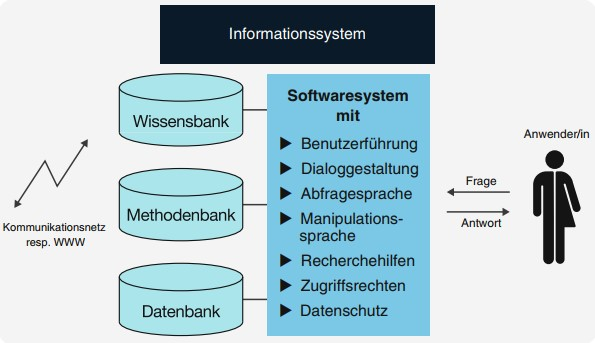
\includegraphics[width=0.7\textwidth]{Bilder/Informationssystem.jpg}
 \vspace{0em}
 \caption[Informationssystem]{Architektur und Komponenten eines Informationssystems  \cite[S. 3]{sqlnosql}}\label{fig:Informationssystem}
\end{figure}

\paragraph*{Datenbankmanagementsysteme}
Ein Datenbanksystem (\textit{engl. database management system}, DBMS) dient der Speicherung und Abfrage von Daten und besteht aus einer Speicher- und Verwaltungskomponente. Die Speicherungskomponente umfasst alle Daten, welche in einer organisierten Form abgespeichert werden sowie deren Beschreibung. Um die Daten und Informationen verändern und auswerten zu können bedarf es einer Abfrage- und Manipulationssprache, die die Verwaltungskomponente darstellt. Die Zugriff- und Bearbeitungsrechte werden ebenfalls von der Verwaltungskomponente verwaltet. In der Praxis kommen häufig SQL-Datenbanken (\textit{Structured Query Language}) zum Einsatz. Sind Datenbestände heterogener Natur und müssen in Echtzeit verarbeitet werden, dann sind SQL-Datenbanken ungeeignet. Für solche Anwendungsfälle bieten sich Lösung im Rahmen von Big Data oder Hybridlösungen an. Datenverwaltungslösungen im Rahmen von Big Data sind No-SQL Datenbanken (not only SQL-Datenbanken) \cite[S. 2 f.]{sqlnosql}.

\paragraph{SQL-Datenbanken}

SQL-Datenbanken sammeln Daten bzw. Informationen in Tabellen. Diese Tabellen können miteinander in Beziehung stehen. Aus diesem Grunde werden SQL-Datenbanken auch relationale Datenbanken genannt. In der Abbildung \ref{fig:tabellengeruest} ist eine Tabelle abgebildet, die den Namen MITARBEITER trägt. Tabellen bestehen aus Schlüsselmerkmalen und Attributen. Schlüsselmerkmale dienen der \textbf{eindeutigen} Identifikation. Ein Merkmal oder Attribut ordnet jedem Eintrag einer Tabelle einen bestimmten Datenwert aus einem vordefinierten Wertebereich (\textit{engl. domain}) zu. Somit kann jeder Mitarbeiter, der eindeutig mit der Mitarbeiter ID identifiziert werden kann, mit Namen und Ort eingetragen und in der Tabelle gefunden werden. Als Schlüsselmerkmal bietet sich demnach die Mitarbeiter ID (\emph{M\#}) an. Die minimale Schlüsselkombination wird in diesem Beispiel durch den \textbf{Identifikationsschlüssel} \emph{M\#} repräsentiert. Schlüsselkombinationen haben einen \textbf{Minimalitätsanspruch}. In diesem Fall darf kein Schlüssel oder Kombination gestrichen werden, ohne dass die eindeutige Identifikation verloren geht. Ein Schlüssel ist mit den Forderungen der \textbf{Minimalität} und \textbf{Eindeutigkeit} vollständig charakterisiert. Datenwerte dürfen mehrfach vorkommen, siehe Abbildung \ref{fig:auspraegungen}. Eine komplette Zeile einer Tabelle wird Datensatz bzw. Tupel genannt und beschreibt ein Objekt in einer Tabelle (ID, Name, Adresse usw.) \cite[S. 3 ff.]{sqlnosql}.\\

Die Anzahl an Spalten und Zeilen ist unbegrenzt. Die Benennung von Tabellen und Merkmalen sowie der Identifikationsschlüssel bzw. Schlüsselkombination muss eindeutig sein. Mathematisch ist eine Relation R, die diesen Anforderung erfüllt, eine Teilmenge aus dem kartesischen Produkt von Wertebereichen $\mathrm{R} \subseteq \mathrm{D}_1\cdot \mathrm{D}_2\cdot...\,\mathrm{D_n}$ mit $\mathrm{D_i}$ als Wertbereich des i-ten Merkmals \cite[S. 3 ff.]{sqlnosql}.



\begin{figure}[h!] % Relationsmodell
\centering
%\hspace{0em}
\captionsetup{position=bottom}
     \subfloat[][Tabellengerüst\label{fig:tabellengeruest}]{%
       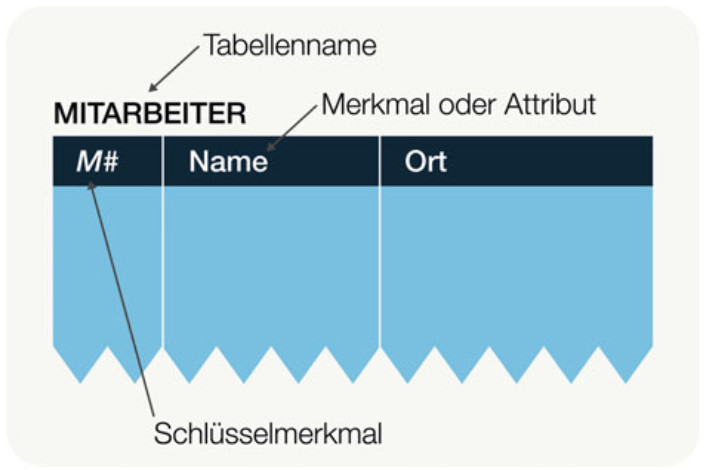
\includegraphics[width=0.40\textwidth,]
       {Bilder/relationstabelle.jpg} %{Bilder/LabVIEW_serialport/}
     }
\hspace{1,5em}%
%\hfill     
    \subfloat[][Ausprägungen\label{fig:auspraegungen}]{%
       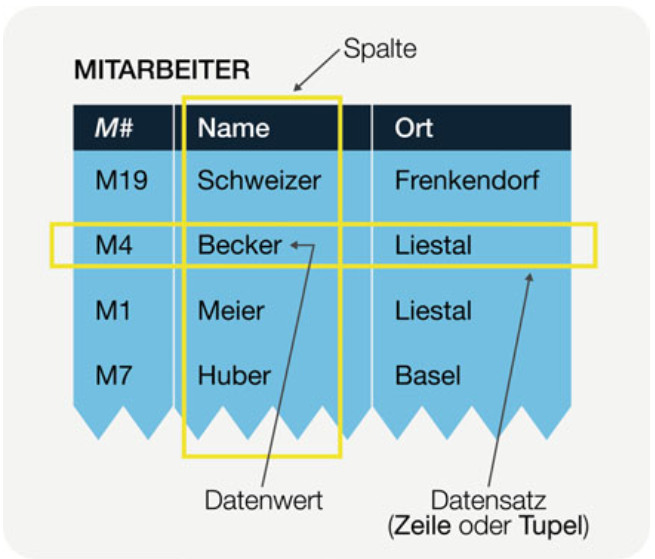
\includegraphics[width=0.40\textwidth]
      {Bilder/relationstabelle_gefuellt.jpg}
      }
\caption[Relationenmodell: Tabellengerüst und Ausprägung einer SQL-Tabelle]{Relationenmodell: Tabellengerüst und Ausprägung einer am Beispiel einer \mbox{MITARBEITER Tabelle}}
\label{fig:relationenmodell}
   \end{figure} 

Ein Tupel r ist demnach ($\mathrm{r} = \mathrm{d}_1 ,\, \mathrm{d}_2 ,...,\,\mathrm{d_n}$). Tupelredundanzen sind aufgrund des Teilmengenbegriffs nicht erlaubt, d.h. $\mathrm{R}=\{\mathrm{r}_1 , \, \mathrm{r}_2 , \, ... , \,\mathrm{r_n}\}$

\footnotesize \singlespacing
\noindent \textbf{Anmerkung:} Beim programmieren sind Tupel unveränderbare, schreibgeschützte Arrays!
\normalsize \onehalfspacing

\subparagraph*{Strukturierte Abfragesprache SQL}

\textit{SQL} (\textit{Structured Query Language}) ist eine \textit{deskriptive} von ANSI und ISO genormte Abfrage- und Manipulationssprache für Tabellen. In der Abbildung \ref{fig:sql} ist ein Beispiel einer Abfrage. unter der Tabelle MITARBEITER ist die Abfrage in natürlicher Sprache (<<Selektiere den ... wohnen>>) zu sehen. Das Resultat der Abfrage sollen alle Namen/Personen die den Wohnort Liestal angegeben haben sein. Die Formulierung einer Abfrage genügt dem Schema SELECT-FROM-WHERE. Eine Formulierung in SQL sieht wie auf Abbildung \ref{fig:sql} zu erkennen folgt aus \cite[S. 6 ff.]{sqlnosql}:

\begin{table}[h!]
\centering
\begin{tabular}{r|l}
SELECT & Name \\
FROM & MITARBEITER \\
WHERE & Ort = 'Liestal' \\
\end{tabular}
\end{table}

\begin{figure}[] %SQL 
\centering
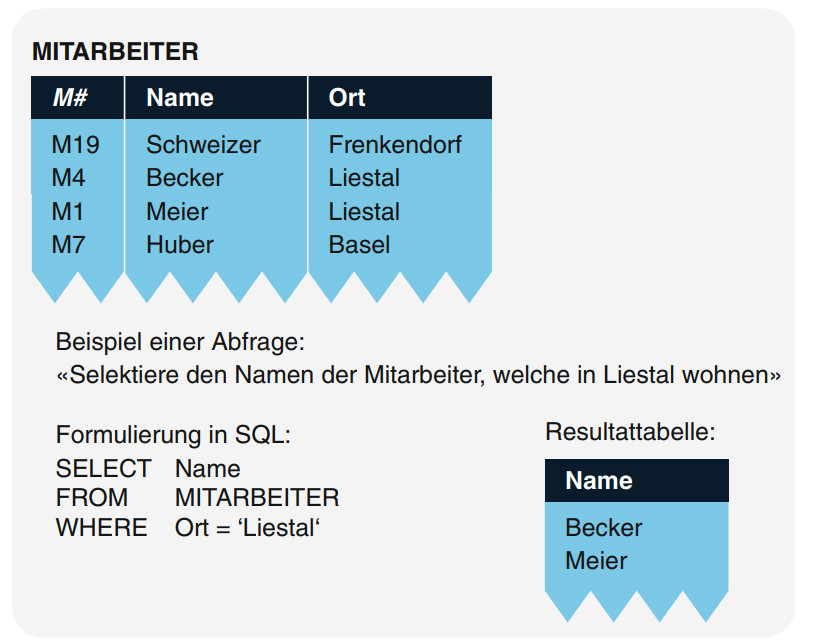
\includegraphics[width=0.6\textwidth]{Bilder/SQL.jpg}
\vspace{0em}
 \caption[]{Formulierung einer SQL Abfrage}\label{fig:sql} %\ref{}
\end{figure}

Für tiefgreifendes Wissen bezüglich SQL-Datenbanken muss auf Fachliteratur wie \cite{sqlnosql} verwiesen werden.

\paragraph{Big Data}

Datenbestände die mit den herkömmlichen technischen Lösungen (SQL-Datenbanken) aufgrund vom sehr hohem Datenvolumen, einer heterogenität von Daten und der Notwendigkeit diese in Echtzeit bei einer hinreichender Geschwindigkeit zu verarbeiten nicht mehr zu handhaben sind, werden unter dem Begriff von \textit{Big Data} zusammengefasst. Der Begriff \textit{Big Data} ist nicht klar definiert. Datenspezialisten wie die Gartner Group definiert Big Data in ihrem \emph{\glqq Information Technology Glossary\grqq{}}mit dem Vorhandensein von mindestens drei \texttt{V}'s \cite[S. 11]{sqlnosql}:\\

\glqq \textbf{Big data} is high-\texttt{v}olume, high-\texttt{v}elocity and/or high-\texttt{v}ariety information assets that demand cost-effective, innovative forms of information processing that enable enhanced insight, decision making, and process automation.\grqq, \cite{BigData}. \\

Wie bereits in Kapitel \ref{sec:Informationsmanagementsysteme} erläutert sind Informationen entscheidend für die Konkurrenzfähigkeit von Unternehmen in vielen Branchen. Die Gartner Group bezeichnet Informationen sogar als \textit{Vermögenswert} oder \textit{Informationskapital} (\textit{engl. information asset}).

Eine Präzisierung der drei \texttt{V}'s laut\cite{sqlnosql} ist folgende: 

\begin{itemize}[leftmargin=*,labelsep=-\mylen]
\item \textbf{Velocity}: Datenströme sollen in Echtzeit analysiert und ausgewertet werden können,
\item \textbf{Volume}: Umfangreiche Datenbestände bis zum Zettabytebereich (1 Zettabyte $+10^{12}$ GB),
\item \textbf{Variety}: Strukturierte, semi-strukturierte und unstrukturierte Multimedia-Daten (Texte, Bilder, Grafiken, Audio Videos) sollen gespeichert werden können.
\end{itemize}

Zuletzt bleibt noch die Information als \texttt{V}ermögenswert (\textit{engl. \texttt{v}alue}) und die Aussagekraft bzw. Wahrhaftigkeit (\textit{engl. \texttt{v}eracity}) der Daten bzw. Auswertungsergebnisse. Da die Daten im Rahmen von \textit{Big Data} heterogener Natur in Art und Präzision sind, müssen spezielle Algorithmen für hinreichende Ergebnisse angewendet werden.  


\subsubsection{PERA-ICS Modell}

Die \textbf{P}urdue \textbf{E}nterprise \textbf{R}eference \textbf{A}rchitecture (PERA) wurde Anfang 1990 entworfen, um Automatisierungsnetze zu beschreiben und zu unterteilen. Des Weiteren dient es unter anderem dazu, den Schutz von industriellen Steuerungs- und Automatisierungsnetze, vor Hackern, zu gewährleisten. Klassisch wird das ICS-Modell (\textbf{I}ndustrial \textbf{C}ontrol \textbf{S}ystem) in fünf Ebenen (\textit{engl. Level}; siehe Abbildung~\ref{pera_modell}) unterteilt. Die oberen zwei Hierarchieebenen sind, gemäß PERA-ICS, von Level 3 bis \textcolor{black!60}{Level 0}, aus sicherheitstechnischen Gründen, physisch voneinander getrennt \cite[S. 15 ff.]{ics_kompendium}. Auf die Funktionen und Komponenten, wie z.B. HMI/BuB (\textbf{H}uman-\textbf{M}achine-\textbf{I}nterface = \textbf{B}edienung \textbf{u}nd \textbf{B}eobachtung), \textit{\textbf{M}anufacturing \textbf{E}xecution \textbf{S}ystem} (MES) oder \textit{\textbf{M}anufacturing \textbf{O}perations \textbf{M}anagement} (MOM) und \textit{\textbf{E}nterprise \textbf{R}essource \textbf{P}laning} (ERP) Systeme usw., die auf den Leveln vorhanden sind, wird im Rahmen dieser Arbeit nicht eingegangen.

\begin{figure} % PERA Model
\begin{center}
\begin{tikzpicture}[
	scale=0.75,
	start chain=1 going below, 
	start chain=2 going right,
	node distance=1mm,
	desc/.style={
		scale=0.85,
		on chain=2,
		rectangle,
		rounded corners,
		draw=black, 
		very thick,
		text centered,
		text width=12cm,
		minimum height=12mm,
		fill=blue!30
		},
	it/.style={
		fill=blue!10
	},
	level/.style={
		scale=0.85,
		on chain=1,
		minimum height=12mm,
		text width=2cm,
		text centered
	},
	every node/.style={font=\sffamily}
]

% Levels
\node [level] (Level 5) {Level 5};
\node [level] (Level 4) {Level 4};
\node [level] (Level 3) {Level 3};
\node [level] (Level 2) {Level 2};
\node [level] (Level 1.5) { };
\node [level] (Level 1) {Level 1};
\node [level] (Level 0) {\textcolor{black!60}{Level 0}};

% Descriptions
\chainin (Level 5); % Start right of Level 5
% IT levels
\node [desc, it] (Archives) {Produktionsführung: ERP, Finanzen uvm.};
\node [desc, it, continue chain=going below] (ERP) {Betriebssführung: MES, Engineering/Planung uvm.};
% ICS levels
\node [desc] (Operations) {Einrichtung zur Prozessführung};
\node [desc] (Supervisory) {Realtime Prozessführung};
\node [desc, text width=3.5cm, xshift=4.25cm] (PLC) {Kommunikation z.B. via RS-232};
%\node [desc, text width=3.5cm, xshift=-4.5cm] (SIS) {Safety Instrumented Systems};
\node [desc, xshift=-4.25cm] (SIS) {Prozessführung im Feld};
\node [desc] (IO) {Materieller Produktionsprozess};
\end{tikzpicture}

\vspace{0,5em}
\caption[]
{ICS-PERA Model, angelehnt an der Grafik des Bundesamtes für Sicherheit in der Informationstechnik des ICS-Kompendiums (vgl. Abbildung \ref{fig:Hierarchische_Gliederung_gem_ICS} im Anhang ; \cite[S. 18]{ics_kompendium})}
\label{pera_modell}
\end{center}
\end{figure}

\paragraph*{\textcolor{black!60}{Level 0}} Gemäß des ICS-Kompendiums des Bundesamtes für Sicherheit in der Informationstechnik, befindet sich vor dem Level 1 der \textbf{materielle Produktionsprozess} \cite[S. 18]{ics_kompendium}. In dem ICS-Kompendium ist es nicht gelabelt, doch in vielen anderen Quellen wird dieses mit \textcolor{black!60}{Level 0} deklariert.

\paragraph*{Level 1} Level 1 ist die \textbf{Prozessführung im Feld} (\textit{engl. Basic Control}). Daten und Signale werden auf dieser Ebene in Realtime generiert und erfasst. Die Ausführung der Steuer- und Regelung physischer Prozesse geschieht auf dieser Ebene. Als Beispiele, für die Infrastruktur dieser Ebene , können Remote I/O (ggf. mit Signalvorverarbeitung, dann spricht man von RTU), Interface-Bausteine zur Signalkonditionierung, Switches bei Verwendung von Feldbus Lösungen genannt werden \cite[S. 18]{ics_kompendium}.

\paragraph*{Level 2} Komponenten der \textbf{Realtime Signalverarbeitung}, im Sinne der Darstellung der automatisierten Funktionen sind dem Level 2 zugeordnet. Beispiele können Zustände der Komponenten der Feldebene sein. Als Beispiele können Füllstände, Motoren (an/aus; Leistungsabnahme), Ventilstellungen uvm. genannt werden.  Stellvertretend für die Kommunikation zwischen diesem und Level 1 ist die \textbf{RS-232}-Schnittstelle aufgelistet \cite[S. 19]{ics_kompendium}.

\paragraph*{Level 3} \textbf{Einrichtungen zur Prozessführung} (\textit{engl. Supervisory Control}) sind dem Level 3 zugeordnet. Diese Einrichtungen sind für die Prozessführung notwendig, jedoch werden keine Daten in Echtzeit verarbeitet. Als Beispiele können \textit{HMI/BUB}, produktbezogene Engineering- und Wartungsstationen, Messwert- und Prozessdatenarchivserver genannt werden. Diese Komponenten sind wichtig, jedoch in Bezug auf das Zeitverhalten oder die Verfügbarkeit unkritischer als Komponenten der Level 1 und 2. Softwareupdates von Komponenten die dieser Ebene zugeordnet sind, werden restriktiv behandelt, da diese die Schnittstelle für die Komponenten der Level 1 und 2 sind, dessen Verfügbarkeit in Realtime zwingend erforderlich ist \cite[S. 19 f.]{ics_kompendium}.

\paragraph*{Level 4} Es ist zu erkennen, dass das 4. Level der \textbf{Betriebsführung} entspricht. Betriebsführung wird oftmals auch \textbf{operatives Management} genannt.  Level 4 sind Funktionen und Komponenten wie, MES oder MOM, Engineering/Planung und lokale Office IT, zuzuordnen \cite[S. 20]{ics_kompendium}.

\paragraph*{Level 5} Hinter Level 5 verbirgt sich die \textbf{Produktionsführung}, mit Funktionen wie ERP Anbindung (interagiert oftmals mit MES Systeme (Level 4) via XML/B2MML, siehe Abschnitt \ref{sec:isa_95}, Inter-/Intranet Zugang, Remote Access Einrichtungen (zur Fernwartung) \cite[S. 20 f.]{ics_kompendium}.


\subsubsection{ISA-S95} 
\label{sec:isa_95}

Unternehmen sind sozio-ökonimische Systeme. Um global wettbewerbsfähig zu bleiben, ist Flexibilität und das Anwenden effizienterer Methoden, als Unternehmen aus \glqq Billiglohnländern\grqq, ein muss. Um die Wettbewerbsfähigkeit zu gewährleisten, ist ein System notwendig, welches die gesamte Wertschöpfungskette abbilden kann.  Ein Austausch von Daten, bspw. zwischen der Supply Chain und der Produktion wird dadurch ermöglicht. \\

Unternehmen können hierarchisch, nach Level, unterteilt werden. Die \textbf{I}nternational \textbf{S}ociety of \textbf{A}utomation, kurz ISA, hat 1995 einen \texttt{S}tandard etabliert, der Terminologie und abstrakte Modelle für den effizienten Datenaustausch zwischen Systemen verschiedener Hierarchiestufen ermöglicht. Ein effizienter Datenfluss zwischen verschiedenen Unternehmenssystemen, wie ERP (Level 5) oder MES (Level 4), wird durch den ISA-95 \texttt{S}tandard ermöglicht. ISA-\textcolor{blue}{S}95 definiert Terminologie und einheitliche Modelle, um die Kommunikation zwischen sämtlichen Kontroll- und Unternehmenssystemen zu verbessern. Die Aktivitäten innerhalb eines Unternehmens werden nach dem PERA-ICS Modell unterteilt. Die Level \textcolor{black!60}{0},\,1 und 2 decken damit die Aktivitäten der Produktion ab. \textbf{Demnach enthält der Standard alles, was Unternehmen benötigen, um sich ihr \underline{MES} entwickeln zu können} \cite{processisa95}. \\

ISA-\textcolor{blue}{S}95 definiert keine Datentypen. Die Definition, in welcher Form Daten für die Datenkommunikation vorzuliegen haben, übernimmt B2MML - \textbf{B}usiness \textbf{To} \textbf{M}anufacturing \textbf{M}arkup \textbf{L}anguage. In \textbf{X}ML-\textbf{S}chema \textbf{D}efiniton (XSD) wird die Datenstruktur festgelgelegt \cite{processisa95}. Die XSD-Dateien dienen somit als Referenz, zur Validierung der XML-Dateien, mit denen im Unternehmen operiert wird und können sich demnach, je nach Unternehmen und Unternehmensfunktion, unterscheiden. Auf der Seite des ISA-\textcolor{blue}{S}95 gibt es diverse B2MML XML-Schemata frei zum downloaden \cite{isa_s95}. Auf XML wird im Rahmen dieser Arbeit nicht weiter eingegangen. ISA-\textcolor{blue}{S}95 besteht aus den folgenden fünf Parts. 

\paragraph*{Part 1} Der erste Part, \glqq Models and Terminology (veröffentlicht 2000)\grqq{}, kann als Leitfaden dienen, um Schnittstellen zwischen Prozess- und Produktions-/ Leitsystemen zu definieren \cite{isa_s95}.

\paragraph*{Part 2} In Part zwei, \glqq  Object Model Attributes (veröffentlicht 2001)\grqq , werden in Kombination mit Part 1 die Inhalte der Schnittstellen zwischen den Steuerungsfunktionen in der Produktion und der Unternehmensführung definiert \cite{isa_s95}.

%ANSI / ISA-95.00.02-2001, Enterprise-Control-Systemintegration Teil 2: Objektmodellattribute bestehen aus Attributen für jedes in Teil 1 definierte Objekt. Die Objekte und Attribute von Teil 2 können für den Informationsaustausch zwischen verwendet werden verschiedene Systeme, aber diese Objekte und Attribute können auch als Grundlage für relationale Datenbanken verwendet werden. ANSI / ISA-95 - https://de.qaz.wiki/wiki/ANSI/ISA-95 

%https://de.qaz.wiki/wiki/ANSI/ISA-95

\paragraph*{Part 3} Der dritte Part, \glqq Models of Manufacturing Operations\grqq , konzentriert sich auf die Produktions- und MES Ebene (Level 4). Der Fokus liegt auf den Aktivitäten und Funktionen von Produktion, Wartung, Lagerhaltung und Qualitätskontrolle \cite{isa_s95}.

\paragraph*{Part 4} \glqq Object Models and Attributes of Manufacturing Operations Management\grqq{} dient als Basis für das Design und die Implementierung von Schnittstellenstandards \cite{isa_s95}.

\paragraph*{Part 5} Part 5, \glqq Business to manufacturing transactions\grqq , nutzt die abstrakten Modelle aus Part 1 sowie 2 und definiert Transaktionsmodelle für den Informations-/Datenaustausch \cite{isa_s95}.

\subsubsection{B2MML}

Das \textbf{W}orld \textbf{B}atch \textbf{F}orum (WBF) hat, in Bezug auf ISA-\texttt{S}95, die \textbf{B}usiness \textbf{To} \textbf{M}anufacturing \textbf{M}arkup \textbf{L}anguage (B2MML) etabliert. WBF ist ein Teil der \textbf{M}anufacturing \textbf{E}nterprise \textbf{S}olutions \textbf{A}ssociation (MESA). ISA-\texttt{S}95 gibt die Terminologie und die abstrakten Modelle vor und das WBF hat mit B2MML einen Datentyp bereit gestellt. B2MML und XML sind textbasierte Formate und lassen sich somit von Menschen lesen (vgl. Ausschnitt der ProcessSegment XSD in der Abbildung \ref{fig:processsegment} im Anhang). B2MML ist eine abgewandelte Form des ursprünglichen XML Formats. Für Batch und kontinuierliche Prozesse hat das WBF neben dem B2MML ebenfalls BatchML etabliert. Um die Datenstruktur besser zu verstehen, wird ein fiktiver (siehe Abbildung \ref{fig:fiktiver_prozess}), jedoch plausibler Prozess und die Prozesssegment XSD (siehe Abbildung \ref{fig:processsegment_visu}), in visualisierter Form, des \textit{Methods Artikel} \cite{ISA-S95_sharing_data} verwendet. Im Rahmen dieser Erläuterung, soll diese Prozesskette einen Wirbelschichtreaktionsprozess darstellen.

\begin{figure}[h!] %[htbp!] 
\centering
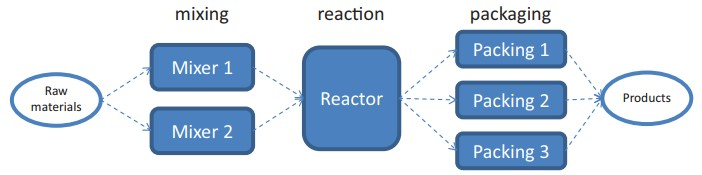
\includegraphics[width=0.8\textwidth]{Bilder/fiktiver_artikel.jpg}
\vspace{0em}
 \caption[]{Fiktiver Prozess des Artikels \cite[S. 3]{ISA-S95_sharing_data}}\label{fig:fiktiver_prozess}
\end{figure}

In der Abbildung \ref{fig:fiktiver_prozess} ist eine Schema einer Prozesskette eines Batchprozess; vom Rohmaterial, bis zum fertigen Produkt; abgebildet. Die verfahrenstechnischen Schritte sind das homogenisieren mittels Mixer (zwei verfügbar), der Reaktor, in dem die chemische Reaktion stattfindet und die Verpackung, wofür drei Packstationen oder Abfüllungen zur Verfügung stehen. In der Abbildung \ref{fig:processsegment_visu} ist das Datenformat der Prozesssegment XSD, in visualisierter Form, dargestellt. Es ist eine hierarchische Struktur zu erkennen. Der Hierarchieursprung wird \textbf{Wurzelelement} genannt und ist in dieser XSD Visualisierung \textit{ProcessSegmentInformation}. Jede B2MML oder BatchML Datei hat einen identischen Aufbau. \textit{ProcessSegmentInformation} ID (1) könnte z.B. \glqq Wirbelschichtrreaktionsprozess\grqq{} heißen. Demnach gäbe es drei \textit{ProcessSegment} ID's (2); für \glqq mixing\grqq, \glqq reaction\grqq, \glqq packaging\grqq. Da sich Equipment des gleichen Typs, z.B. Mixer, in ihrer Funktion unterscheiden können, empfiehlt es sich ggf. \textit{EquipmentClassID's} (3) zu vergeben. Des Weiteren können Abhangigkeiten (\textit{engl. Dependency}) zwischen den \textit{ProcessSegments} existieren, die unter dem Reiter \textit{SegmentDependency} (4 - 6) genau definiert werden können. 

\begin{figure}[h!] %[htbp!] 
\begin{flushleft}
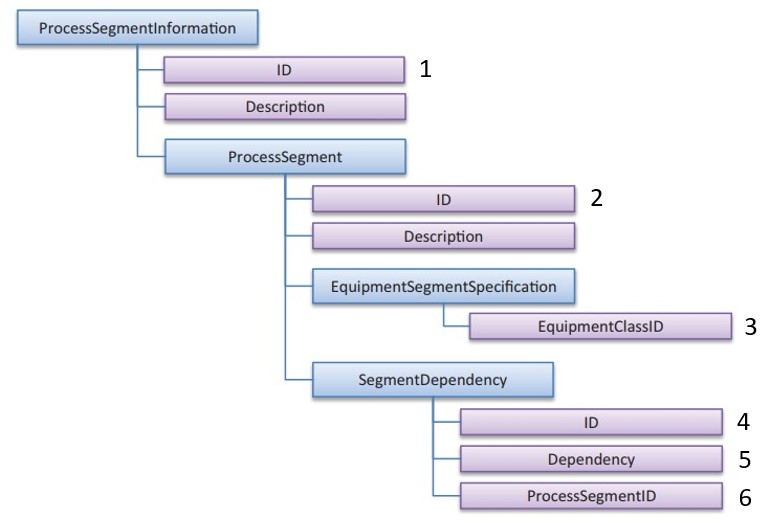
\includegraphics[width=1\textwidth]{Bilder/processsegment_visu.jpg}
\vspace{0em}
 \caption[]{Prozesssegment Informationen \cite{ISA-S95_sharing_data}}\label{fig:processsegment_visu}
\end{flushleft}
\end{figure}
In der folgenden Liste ist ein Teil der vordefinierten, der auf der MESA frei erhältlichen XSD-Files, nach Erstellung eines Accounts, aufgelistet \cite{B2MML}:

\begin{enumerate}[label = \textbullet , itemsep = -0.2em]
\item ProcessSegmentInformation (B2MML-V0600-ProcessSegment.xsd)
\item EquipmentInformation (B2MML-V0600-Equipment.xsd)
\item MaterialInformation (B2MML-V0600-Material.xsd)
\item PersonnelInformation (B2MML-V0600-Personnel.xsd)
\item OperationsCapability (B2MML-V0600-OperationsCapability.xsd)
\item OperationsDefinitionInformation (B2MML-V0600-OperationsDefinition.xsd)
\item OperationsSchedule (B2MML-V0600-OperationsSchedule.xsd)
\item OperationsResponse (B2MML-V0600-OperationsPerformance.xsd)
\item BatchML-V0600-BatchInformation.xsd
\item BatchML-V0600-BatchProductionRecord.xsd
\item BatchML-V0600-GeneralRecipe.xsd
\end{enumerate}
 

